\documentclass[twoside]{book}

% Packages required by doxygen
\usepackage{fixltx2e}
\usepackage{calc}
\usepackage{doxygen}
\usepackage[export]{adjustbox} % also loads graphicx
\usepackage{graphicx}
\usepackage[utf8]{inputenc}
\usepackage{makeidx}
\usepackage{multicol}
\usepackage{multirow}
\PassOptionsToPackage{warn}{textcomp}
\usepackage{textcomp}
\usepackage[nointegrals]{wasysym}
\usepackage[table]{xcolor}

% Font selection
\usepackage[T1]{fontenc}
\usepackage[scaled=.90]{helvet}
\usepackage{courier}
\usepackage{amssymb}
\usepackage{sectsty}
\renewcommand{\familydefault}{\sfdefault}
\allsectionsfont{%
  \fontseries{bc}\selectfont%
  \color{darkgray}%
}
\renewcommand{\DoxyLabelFont}{%
  \fontseries{bc}\selectfont%
  \color{darkgray}%
}
\newcommand{\+}{\discretionary{\mbox{\scriptsize$\hookleftarrow$}}{}{}}

% Page & text layout
\usepackage{geometry}
\geometry{%
  a4paper,%
  top=2.5cm,%
  bottom=2.5cm,%
  left=2.5cm,%
  right=2.5cm%
}
\tolerance=750
\hfuzz=15pt
\hbadness=750
\setlength{\emergencystretch}{15pt}
\setlength{\parindent}{0cm}
\setlength{\parskip}{3ex plus 2ex minus 2ex}
\makeatletter
\renewcommand{\paragraph}{%
  \@startsection{paragraph}{4}{0ex}{-1.0ex}{1.0ex}{%
    \normalfont\normalsize\bfseries\SS@parafont%
  }%
}
\renewcommand{\subparagraph}{%
  \@startsection{subparagraph}{5}{0ex}{-1.0ex}{1.0ex}{%
    \normalfont\normalsize\bfseries\SS@subparafont%
  }%
}
\makeatother

% Headers & footers
\usepackage{fancyhdr}
\pagestyle{fancyplain}
\fancyhead[LE]{\fancyplain{}{\bfseries\thepage}}
\fancyhead[CE]{\fancyplain{}{}}
\fancyhead[RE]{\fancyplain{}{\bfseries\leftmark}}
\fancyhead[LO]{\fancyplain{}{\bfseries\rightmark}}
\fancyhead[CO]{\fancyplain{}{}}
\fancyhead[RO]{\fancyplain{}{\bfseries\thepage}}
\fancyfoot[LE]{\fancyplain{}{}}
\fancyfoot[CE]{\fancyplain{}{}}
\fancyfoot[RE]{\fancyplain{}{\bfseries\scriptsize Generated by Doxygen }}
\fancyfoot[LO]{\fancyplain{}{\bfseries\scriptsize Generated by Doxygen }}
\fancyfoot[CO]{\fancyplain{}{}}
\fancyfoot[RO]{\fancyplain{}{}}
\renewcommand{\footrulewidth}{0.4pt}
\renewcommand{\chaptermark}[1]{%
  \markboth{#1}{}%
}
\renewcommand{\sectionmark}[1]{%
  \markright{\thesection\ #1}%
}

% Indices & bibliography
\usepackage{natbib}
\usepackage[titles]{tocloft}
\setcounter{tocdepth}{3}
\setcounter{secnumdepth}{5}
\makeindex

% Hyperlinks (required, but should be loaded last)
\usepackage{ifpdf}
\ifpdf
  \usepackage[pdftex,pagebackref=true]{hyperref}
\else
  \usepackage[ps2pdf,pagebackref=true]{hyperref}
\fi
\hypersetup{%
  colorlinks=true,%
  linkcolor=blue,%
  citecolor=blue,%
  unicode%
}

% Custom commands
\newcommand{\clearemptydoublepage}{%
  \newpage{\pagestyle{empty}\cleardoublepage}%
}

\usepackage{caption}
\captionsetup{labelsep=space,justification=centering,font={bf},singlelinecheck=off,skip=4pt,position=top}

%===== C O N T E N T S =====

\begin{document}

% Titlepage & ToC
\hypersetup{pageanchor=false,
             bookmarksnumbered=true,
             pdfencoding=unicode
            }
\pagenumbering{roman}
\begin{titlepage}
\vspace*{7cm}
\begin{center}%
{\Large My Project }\\
\vspace*{1cm}
{\large Generated by Doxygen 1.8.11}\\
\end{center}
\end{titlepage}
\clearemptydoublepage
\tableofcontents
\clearemptydoublepage
\pagenumbering{arabic}
\hypersetup{pageanchor=true}

%--- Begin generated contents ---
\chapter{Hierarchical Index}
\section{Class Hierarchy}
This inheritance list is sorted roughly, but not completely, alphabetically\+:\begin{DoxyCompactList}
\item \contentsline{section}{D\+Bconnect.\+D\+Bconnect}{\pageref{class_d_bconnect_1_1_d_bconnect}}{}
\item \contentsline{section}{history.\+History\+Bean}{\pageref{classhistory_1_1_history_bean}}{}
\item \contentsline{section}{loan.\+Loan\+Bean}{\pageref{classloan_1_1_loan_bean}}{}
\item \contentsline{section}{admin.\+Modify\+Bean}{\pageref{classadmin_1_1_modify_bean}}{}
\item \contentsline{section}{admin.\+Result\+Bean}{\pageref{classadmin_1_1_result_bean}}{}
\item Http\+Servlet\begin{DoxyCompactList}
\item \contentsline{section}{admin.\+Add\+Servlet}{\pageref{classadmin_1_1_add_servlet}}{}
\item \contentsline{section}{admin.\+Check\+Loan\+Servlet}{\pageref{classadmin_1_1_check_loan_servlet}}{}
\item \contentsline{section}{admin.\+Controller\+Servlet}{\pageref{classadmin_1_1_controller_servlet}}{}
\item \contentsline{section}{admin.\+Modify\+Servlet}{\pageref{classadmin_1_1_modify_servlet}}{}
\item \contentsline{section}{admin.\+Remove\+Servlet}{\pageref{classadmin_1_1_remove_servlet}}{}
\item \contentsline{section}{admin.\+Return\+Servlet}{\pageref{classadmin_1_1_return_servlet}}{}
\item \contentsline{section}{admin.\+Search\+Servlet}{\pageref{classadmin_1_1_search_servlet}}{}
\item \contentsline{section}{advanced.\+Advanced\+Search\+Servlet}{\pageref{classadvanced_1_1_advanced_search_servlet}}{}
\item \contentsline{section}{advanced.\+All\+Book\+Servlet}{\pageref{classadvanced_1_1_all_book_servlet}}{}
\item \contentsline{section}{advanced.\+Recommend\+Servlet}{\pageref{classadvanced_1_1_recommend_servlet}}{}
\item \contentsline{section}{advanced.\+Request\+Servlet}{\pageref{classadvanced_1_1_request_servlet}}{}
\item \contentsline{section}{login.\+Login\+Servlet}{\pageref{classlogin_1_1_login_servlet}}{}
\end{DoxyCompactList}
\end{DoxyCompactList}

\chapter{Class Index}
\section{Class List}
Here are the classes, structs, unions and interfaces with brief descriptions\+:\begin{DoxyCompactList}
\item\contentsline{section}{\hyperlink{classadmin_1_1_add_servlet}{admin.\+Add\+Servlet} }{\pageref{classadmin_1_1_add_servlet}}{}
\item\contentsline{section}{\hyperlink{classadvanced_1_1_advanced_search_servlet}{advanced.\+Advanced\+Search\+Servlet} }{\pageref{classadvanced_1_1_advanced_search_servlet}}{}
\item\contentsline{section}{\hyperlink{classadvanced_1_1_all_book_servlet}{advanced.\+All\+Book\+Servlet} }{\pageref{classadvanced_1_1_all_book_servlet}}{}
\item\contentsline{section}{\hyperlink{classadmin_1_1_check_loan_servlet}{admin.\+Check\+Loan\+Servlet} }{\pageref{classadmin_1_1_check_loan_servlet}}{}
\item\contentsline{section}{\hyperlink{classadmin_1_1_controller_servlet}{admin.\+Controller\+Servlet} }{\pageref{classadmin_1_1_controller_servlet}}{}
\item\contentsline{section}{\hyperlink{class_d_bconnect_1_1_d_bconnect}{D\+Bconnect.\+D\+Bconnect} }{\pageref{class_d_bconnect_1_1_d_bconnect}}{}
\item\contentsline{section}{\hyperlink{classhistory_1_1_history_bean}{history.\+History\+Bean} }{\pageref{classhistory_1_1_history_bean}}{}
\item\contentsline{section}{\hyperlink{classloan_1_1_loan_bean}{loan.\+Loan\+Bean} }{\pageref{classloan_1_1_loan_bean}}{}
\item\contentsline{section}{\hyperlink{classlogin_1_1_login_servlet}{login.\+Login\+Servlet} }{\pageref{classlogin_1_1_login_servlet}}{}
\item\contentsline{section}{\hyperlink{classadmin_1_1_modify_bean}{admin.\+Modify\+Bean} }{\pageref{classadmin_1_1_modify_bean}}{}
\item\contentsline{section}{\hyperlink{classadmin_1_1_modify_servlet}{admin.\+Modify\+Servlet} }{\pageref{classadmin_1_1_modify_servlet}}{}
\item\contentsline{section}{\hyperlink{classadvanced_1_1_recommend_servlet}{advanced.\+Recommend\+Servlet} }{\pageref{classadvanced_1_1_recommend_servlet}}{}
\item\contentsline{section}{\hyperlink{classadmin_1_1_remove_servlet}{admin.\+Remove\+Servlet} }{\pageref{classadmin_1_1_remove_servlet}}{}
\item\contentsline{section}{\hyperlink{classadvanced_1_1_request_servlet}{advanced.\+Request\+Servlet} }{\pageref{classadvanced_1_1_request_servlet}}{}
\item\contentsline{section}{\hyperlink{classadmin_1_1_result_bean}{admin.\+Result\+Bean} }{\pageref{classadmin_1_1_result_bean}}{}
\item\contentsline{section}{\hyperlink{classadmin_1_1_return_servlet}{admin.\+Return\+Servlet} }{\pageref{classadmin_1_1_return_servlet}}{}
\item\contentsline{section}{\hyperlink{classadmin_1_1_search_servlet}{admin.\+Search\+Servlet} }{\pageref{classadmin_1_1_search_servlet}}{}
\end{DoxyCompactList}

\chapter{Class Documentation}
\hypertarget{classadmin_1_1_add_servlet}{}\section{admin.\+Add\+Servlet Class Reference}
\label{classadmin_1_1_add_servlet}\index{admin.\+Add\+Servlet@{admin.\+Add\+Servlet}}
Inheritance diagram for admin.\+Add\+Servlet\+:\begin{figure}[H]
\begin{center}
\leavevmode
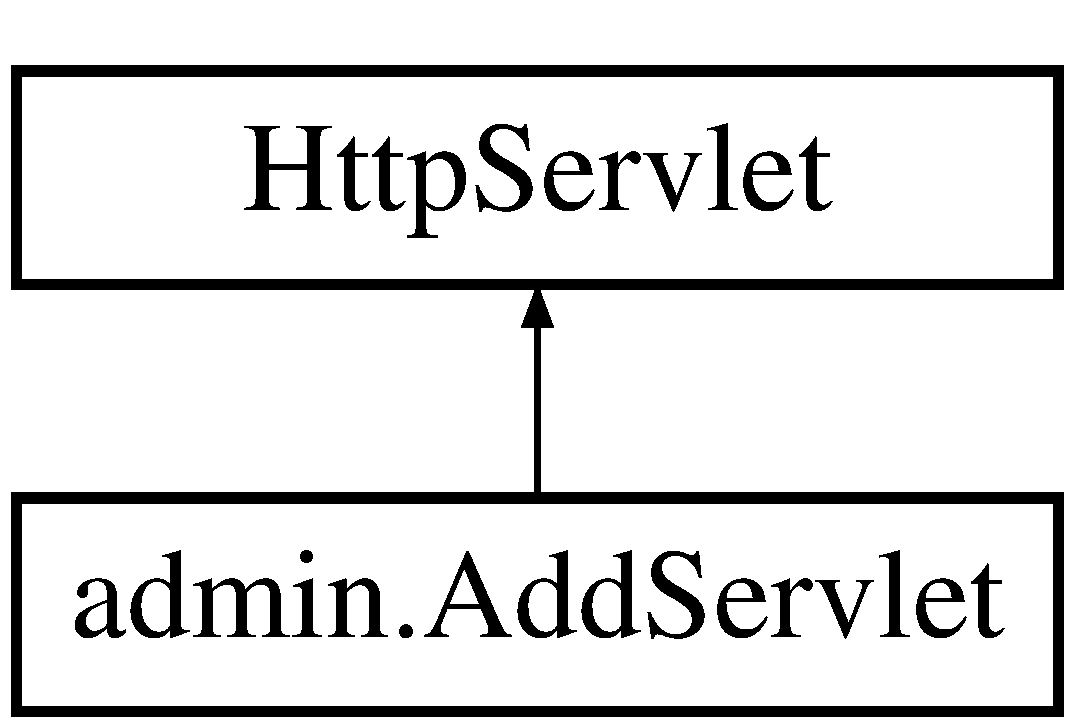
\includegraphics[height=2.000000cm]{classadmin_1_1_add_servlet}
\end{center}
\end{figure}
\subsection*{Public Member Functions}
\begin{DoxyCompactItemize}
\item 
\hyperlink{classadmin_1_1_add_servlet_a8e5e2cb34988a4a3cfbc766448be1fc4}{Add\+Servlet} ()
\end{DoxyCompactItemize}
\subsection*{Protected Member Functions}
\begin{DoxyCompactItemize}
\item 
void \hyperlink{classadmin_1_1_add_servlet_adbc63c3d39dcf577c95795457718f95e}{do\+Get} (Http\+Servlet\+Request request, Http\+Servlet\+Response response)  throws Servlet\+Exception, I\+O\+Exception 
\item 
void \hyperlink{classadmin_1_1_add_servlet_a1297b03c40f87a6dff6f3042448583f6}{do\+Post} (Http\+Servlet\+Request request, Http\+Servlet\+Response response)  throws Servlet\+Exception, I\+O\+Exception 
\end{DoxyCompactItemize}


\subsection{Detailed Description}
Servlet implementation class \hyperlink{classadmin_1_1_add_servlet}{Add\+Servlet} 

\subsection{Constructor \& Destructor Documentation}
\index{admin\+::\+Add\+Servlet@{admin\+::\+Add\+Servlet}!Add\+Servlet@{Add\+Servlet}}
\index{Add\+Servlet@{Add\+Servlet}!admin\+::\+Add\+Servlet@{admin\+::\+Add\+Servlet}}
\subsubsection[{\texorpdfstring{Add\+Servlet()}{AddServlet()}}]{\setlength{\rightskip}{0pt plus 5cm}admin.\+Add\+Servlet.\+Add\+Servlet (
\begin{DoxyParamCaption}
{}
\end{DoxyParamCaption}
)}\hypertarget{classadmin_1_1_add_servlet_a8e5e2cb34988a4a3cfbc766448be1fc4}{}\label{classadmin_1_1_add_servlet_a8e5e2cb34988a4a3cfbc766448be1fc4}
\begin{DoxySeeAlso}{See also}
Http\+Servlet\+::\+Http\+Servlet() 
\end{DoxySeeAlso}


\subsection{Member Function Documentation}
\index{admin\+::\+Add\+Servlet@{admin\+::\+Add\+Servlet}!do\+Get@{do\+Get}}
\index{do\+Get@{do\+Get}!admin\+::\+Add\+Servlet@{admin\+::\+Add\+Servlet}}
\subsubsection[{\texorpdfstring{do\+Get(\+Http\+Servlet\+Request request, Http\+Servlet\+Response response)}{doGet(HttpServletRequest request, HttpServletResponse response)}}]{\setlength{\rightskip}{0pt plus 5cm}void admin.\+Add\+Servlet.\+do\+Get (
\begin{DoxyParamCaption}
\item[{Http\+Servlet\+Request}]{request, }
\item[{Http\+Servlet\+Response}]{response}
\end{DoxyParamCaption}
) throws Servlet\+Exception, I\+O\+Exception\hspace{0.3cm}{\ttfamily [protected]}}\hypertarget{classadmin_1_1_add_servlet_adbc63c3d39dcf577c95795457718f95e}{}\label{classadmin_1_1_add_servlet_adbc63c3d39dcf577c95795457718f95e}
\begin{DoxySeeAlso}{See also}
Http\+Servlet\+::do\+Get(\+Http\+Servlet\+Request request, Http\+Servlet\+Response response) 
\end{DoxySeeAlso}
\index{admin\+::\+Add\+Servlet@{admin\+::\+Add\+Servlet}!do\+Post@{do\+Post}}
\index{do\+Post@{do\+Post}!admin\+::\+Add\+Servlet@{admin\+::\+Add\+Servlet}}
\subsubsection[{\texorpdfstring{do\+Post(\+Http\+Servlet\+Request request, Http\+Servlet\+Response response)}{doPost(HttpServletRequest request, HttpServletResponse response)}}]{\setlength{\rightskip}{0pt plus 5cm}void admin.\+Add\+Servlet.\+do\+Post (
\begin{DoxyParamCaption}
\item[{Http\+Servlet\+Request}]{request, }
\item[{Http\+Servlet\+Response}]{response}
\end{DoxyParamCaption}
) throws Servlet\+Exception, I\+O\+Exception\hspace{0.3cm}{\ttfamily [protected]}}\hypertarget{classadmin_1_1_add_servlet_a1297b03c40f87a6dff6f3042448583f6}{}\label{classadmin_1_1_add_servlet_a1297b03c40f87a6dff6f3042448583f6}
\begin{DoxySeeAlso}{See also}
Http\+Servlet\+::do\+Post(\+Http\+Servlet\+Request request, Http\+Servlet\+Response response) 
\end{DoxySeeAlso}


The documentation for this class was generated from the following file\+:\begin{DoxyCompactItemize}
\item 
Add\+Servlet.\+java\end{DoxyCompactItemize}

\hypertarget{classadvanced_1_1_advanced_search_servlet}{}\section{advanced.\+Advanced\+Search\+Servlet Class Reference}
\label{classadvanced_1_1_advanced_search_servlet}\index{advanced.\+Advanced\+Search\+Servlet@{advanced.\+Advanced\+Search\+Servlet}}
Inheritance diagram for advanced.\+Advanced\+Search\+Servlet\+:\begin{figure}[H]
\begin{center}
\leavevmode
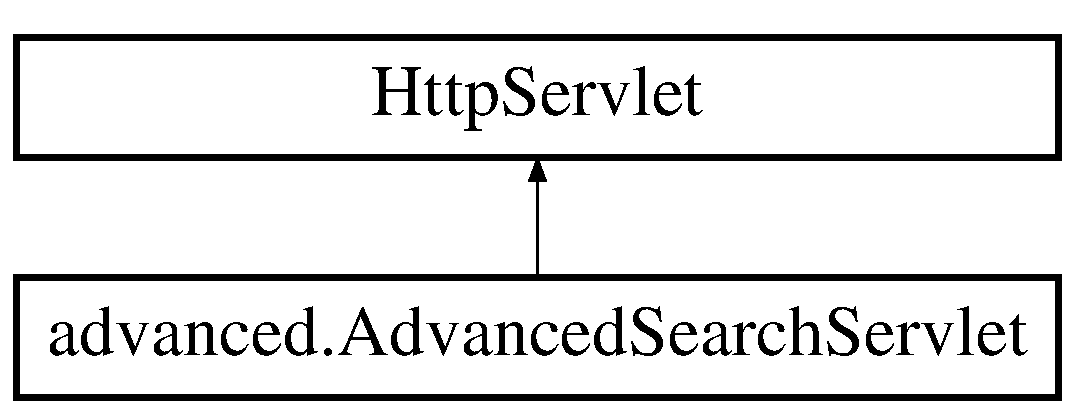
\includegraphics[height=2.000000cm]{classadvanced_1_1_advanced_search_servlet}
\end{center}
\end{figure}
\subsection*{Public Member Functions}
\begin{DoxyCompactItemize}
\item 
\hyperlink{classadvanced_1_1_advanced_search_servlet_acdeda0b58a8e4e4cde7b4755141aa1f5}{Advanced\+Search\+Servlet} ()
\end{DoxyCompactItemize}
\subsection*{Protected Member Functions}
\begin{DoxyCompactItemize}
\item 
void \hyperlink{classadvanced_1_1_advanced_search_servlet_a63c9f9ecb57ff999b13b4ef46764fe39}{do\+Get} (Http\+Servlet\+Request request, Http\+Servlet\+Response response)  throws Servlet\+Exception, I\+O\+Exception 
\item 
void \hyperlink{classadvanced_1_1_advanced_search_servlet_add42de3b72bf474b9462538d39a4f346}{do\+Post} (Http\+Servlet\+Request request, Http\+Servlet\+Response response)  throws Servlet\+Exception, I\+O\+Exception 
\end{DoxyCompactItemize}


\subsection{Detailed Description}
Servlet implementation class \hyperlink{classadvanced_1_1_advanced_search_servlet}{Advanced\+Search\+Servlet} 

\subsection{Constructor \& Destructor Documentation}
\index{advanced\+::\+Advanced\+Search\+Servlet@{advanced\+::\+Advanced\+Search\+Servlet}!Advanced\+Search\+Servlet@{Advanced\+Search\+Servlet}}
\index{Advanced\+Search\+Servlet@{Advanced\+Search\+Servlet}!advanced\+::\+Advanced\+Search\+Servlet@{advanced\+::\+Advanced\+Search\+Servlet}}
\subsubsection[{\texorpdfstring{Advanced\+Search\+Servlet()}{AdvancedSearchServlet()}}]{\setlength{\rightskip}{0pt plus 5cm}advanced.\+Advanced\+Search\+Servlet.\+Advanced\+Search\+Servlet (
\begin{DoxyParamCaption}
{}
\end{DoxyParamCaption}
)}\hypertarget{classadvanced_1_1_advanced_search_servlet_acdeda0b58a8e4e4cde7b4755141aa1f5}{}\label{classadvanced_1_1_advanced_search_servlet_acdeda0b58a8e4e4cde7b4755141aa1f5}
\begin{DoxySeeAlso}{See also}
Http\+Servlet\+::\+Http\+Servlet() 
\end{DoxySeeAlso}


\subsection{Member Function Documentation}
\index{advanced\+::\+Advanced\+Search\+Servlet@{advanced\+::\+Advanced\+Search\+Servlet}!do\+Get@{do\+Get}}
\index{do\+Get@{do\+Get}!advanced\+::\+Advanced\+Search\+Servlet@{advanced\+::\+Advanced\+Search\+Servlet}}
\subsubsection[{\texorpdfstring{do\+Get(\+Http\+Servlet\+Request request, Http\+Servlet\+Response response)}{doGet(HttpServletRequest request, HttpServletResponse response)}}]{\setlength{\rightskip}{0pt plus 5cm}void advanced.\+Advanced\+Search\+Servlet.\+do\+Get (
\begin{DoxyParamCaption}
\item[{Http\+Servlet\+Request}]{request, }
\item[{Http\+Servlet\+Response}]{response}
\end{DoxyParamCaption}
) throws Servlet\+Exception, I\+O\+Exception\hspace{0.3cm}{\ttfamily [protected]}}\hypertarget{classadvanced_1_1_advanced_search_servlet_a63c9f9ecb57ff999b13b4ef46764fe39}{}\label{classadvanced_1_1_advanced_search_servlet_a63c9f9ecb57ff999b13b4ef46764fe39}
\begin{DoxySeeAlso}{See also}
Http\+Servlet\+::do\+Get(\+Http\+Servlet\+Request request, Http\+Servlet\+Response response) 
\end{DoxySeeAlso}
\index{advanced\+::\+Advanced\+Search\+Servlet@{advanced\+::\+Advanced\+Search\+Servlet}!do\+Post@{do\+Post}}
\index{do\+Post@{do\+Post}!advanced\+::\+Advanced\+Search\+Servlet@{advanced\+::\+Advanced\+Search\+Servlet}}
\subsubsection[{\texorpdfstring{do\+Post(\+Http\+Servlet\+Request request, Http\+Servlet\+Response response)}{doPost(HttpServletRequest request, HttpServletResponse response)}}]{\setlength{\rightskip}{0pt plus 5cm}void advanced.\+Advanced\+Search\+Servlet.\+do\+Post (
\begin{DoxyParamCaption}
\item[{Http\+Servlet\+Request}]{request, }
\item[{Http\+Servlet\+Response}]{response}
\end{DoxyParamCaption}
) throws Servlet\+Exception, I\+O\+Exception\hspace{0.3cm}{\ttfamily [protected]}}\hypertarget{classadvanced_1_1_advanced_search_servlet_add42de3b72bf474b9462538d39a4f346}{}\label{classadvanced_1_1_advanced_search_servlet_add42de3b72bf474b9462538d39a4f346}
\begin{DoxySeeAlso}{See also}
Http\+Servlet\+::do\+Post(\+Http\+Servlet\+Request request, Http\+Servlet\+Response response) 
\end{DoxySeeAlso}


The documentation for this class was generated from the following file\+:\begin{DoxyCompactItemize}
\item 
Advanced\+Search\+Servlet.\+java\end{DoxyCompactItemize}

\hypertarget{classadvanced_1_1_all_book_servlet}{}\section{advanced.\+All\+Book\+Servlet Class Reference}
\label{classadvanced_1_1_all_book_servlet}\index{advanced.\+All\+Book\+Servlet@{advanced.\+All\+Book\+Servlet}}
Inheritance diagram for advanced.\+All\+Book\+Servlet\+:\begin{figure}[H]
\begin{center}
\leavevmode
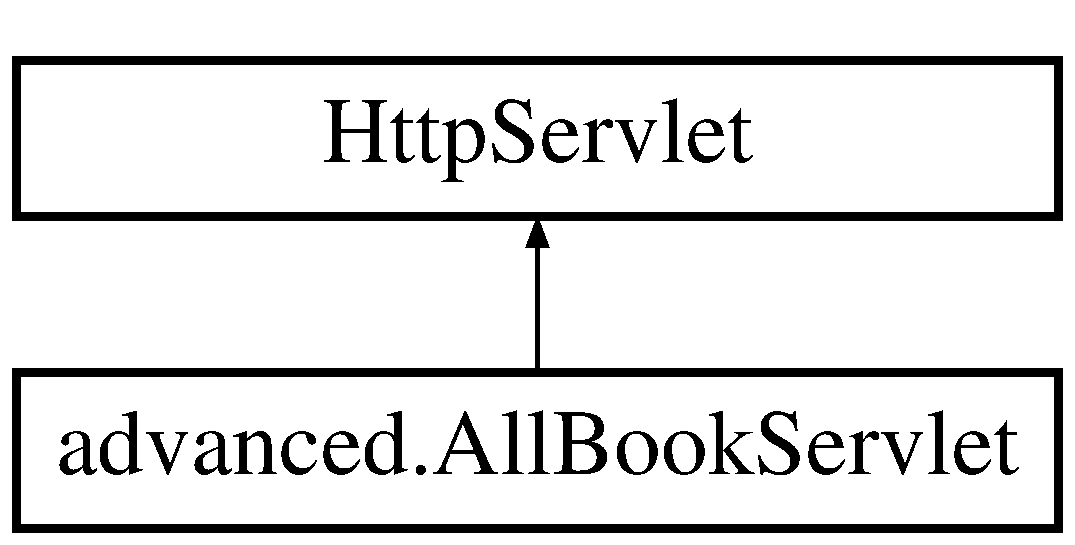
\includegraphics[height=2.000000cm]{classadvanced_1_1_all_book_servlet}
\end{center}
\end{figure}
\subsection*{Public Member Functions}
\begin{DoxyCompactItemize}
\item 
\hyperlink{classadvanced_1_1_all_book_servlet_a37d738fd86cfcf6b73a81044253d0465}{All\+Book\+Servlet} ()
\end{DoxyCompactItemize}
\subsection*{Protected Member Functions}
\begin{DoxyCompactItemize}
\item 
void \hyperlink{classadvanced_1_1_all_book_servlet_a254894253935322173402de169c7d647}{do\+Get} (Http\+Servlet\+Request request, Http\+Servlet\+Response response)  throws Servlet\+Exception, I\+O\+Exception 
\item 
void \hyperlink{classadvanced_1_1_all_book_servlet_a8a5a865de4a130dc91e8354b1a4887ca}{do\+Post} (Http\+Servlet\+Request request, Http\+Servlet\+Response response)  throws Servlet\+Exception, I\+O\+Exception 
\end{DoxyCompactItemize}


\subsection{Detailed Description}
Servlet implementation class \hyperlink{classadvanced_1_1_all_book_servlet}{All\+Book\+Servlet} 

\subsection{Constructor \& Destructor Documentation}
\index{advanced\+::\+All\+Book\+Servlet@{advanced\+::\+All\+Book\+Servlet}!All\+Book\+Servlet@{All\+Book\+Servlet}}
\index{All\+Book\+Servlet@{All\+Book\+Servlet}!advanced\+::\+All\+Book\+Servlet@{advanced\+::\+All\+Book\+Servlet}}
\subsubsection[{\texorpdfstring{All\+Book\+Servlet()}{AllBookServlet()}}]{\setlength{\rightskip}{0pt plus 5cm}advanced.\+All\+Book\+Servlet.\+All\+Book\+Servlet (
\begin{DoxyParamCaption}
{}
\end{DoxyParamCaption}
)}\hypertarget{classadvanced_1_1_all_book_servlet_a37d738fd86cfcf6b73a81044253d0465}{}\label{classadvanced_1_1_all_book_servlet_a37d738fd86cfcf6b73a81044253d0465}
\begin{DoxySeeAlso}{See also}
Http\+Servlet\+::\+Http\+Servlet() 
\end{DoxySeeAlso}


\subsection{Member Function Documentation}
\index{advanced\+::\+All\+Book\+Servlet@{advanced\+::\+All\+Book\+Servlet}!do\+Get@{do\+Get}}
\index{do\+Get@{do\+Get}!advanced\+::\+All\+Book\+Servlet@{advanced\+::\+All\+Book\+Servlet}}
\subsubsection[{\texorpdfstring{do\+Get(\+Http\+Servlet\+Request request, Http\+Servlet\+Response response)}{doGet(HttpServletRequest request, HttpServletResponse response)}}]{\setlength{\rightskip}{0pt plus 5cm}void advanced.\+All\+Book\+Servlet.\+do\+Get (
\begin{DoxyParamCaption}
\item[{Http\+Servlet\+Request}]{request, }
\item[{Http\+Servlet\+Response}]{response}
\end{DoxyParamCaption}
) throws Servlet\+Exception, I\+O\+Exception\hspace{0.3cm}{\ttfamily [protected]}}\hypertarget{classadvanced_1_1_all_book_servlet_a254894253935322173402de169c7d647}{}\label{classadvanced_1_1_all_book_servlet_a254894253935322173402de169c7d647}
\begin{DoxySeeAlso}{See also}
Http\+Servlet\+::do\+Get(\+Http\+Servlet\+Request request, Http\+Servlet\+Response response) 
\end{DoxySeeAlso}
\index{advanced\+::\+All\+Book\+Servlet@{advanced\+::\+All\+Book\+Servlet}!do\+Post@{do\+Post}}
\index{do\+Post@{do\+Post}!advanced\+::\+All\+Book\+Servlet@{advanced\+::\+All\+Book\+Servlet}}
\subsubsection[{\texorpdfstring{do\+Post(\+Http\+Servlet\+Request request, Http\+Servlet\+Response response)}{doPost(HttpServletRequest request, HttpServletResponse response)}}]{\setlength{\rightskip}{0pt plus 5cm}void advanced.\+All\+Book\+Servlet.\+do\+Post (
\begin{DoxyParamCaption}
\item[{Http\+Servlet\+Request}]{request, }
\item[{Http\+Servlet\+Response}]{response}
\end{DoxyParamCaption}
) throws Servlet\+Exception, I\+O\+Exception\hspace{0.3cm}{\ttfamily [protected]}}\hypertarget{classadvanced_1_1_all_book_servlet_a8a5a865de4a130dc91e8354b1a4887ca}{}\label{classadvanced_1_1_all_book_servlet_a8a5a865de4a130dc91e8354b1a4887ca}
\begin{DoxySeeAlso}{See also}
Http\+Servlet\+::do\+Post(\+Http\+Servlet\+Request request, Http\+Servlet\+Response response) 
\end{DoxySeeAlso}


The documentation for this class was generated from the following file\+:\begin{DoxyCompactItemize}
\item 
All\+Book\+Servlet.\+java\end{DoxyCompactItemize}

\hypertarget{classadmin_1_1_check_loan_servlet}{}\section{admin.\+Check\+Loan\+Servlet Class Reference}
\label{classadmin_1_1_check_loan_servlet}\index{admin.\+Check\+Loan\+Servlet@{admin.\+Check\+Loan\+Servlet}}
Inheritance diagram for admin.\+Check\+Loan\+Servlet\+:\begin{figure}[H]
\begin{center}
\leavevmode
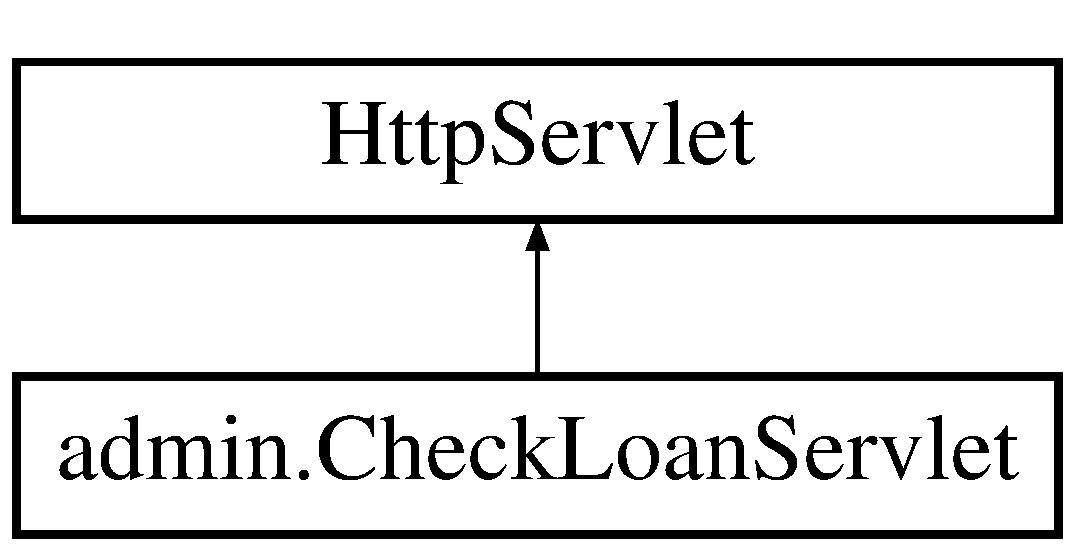
\includegraphics[height=2.000000cm]{classadmin_1_1_check_loan_servlet}
\end{center}
\end{figure}
\subsection*{Public Member Functions}
\begin{DoxyCompactItemize}
\item 
\hyperlink{classadmin_1_1_check_loan_servlet_a4b9867090eb9c2ba7daec58d7c3ec0f5}{Check\+Loan\+Servlet} ()
\end{DoxyCompactItemize}
\subsection*{Protected Member Functions}
\begin{DoxyCompactItemize}
\item 
void \hyperlink{classadmin_1_1_check_loan_servlet_abbe0557187c93d0e806e751add7e5daf}{do\+Get} (Http\+Servlet\+Request request, Http\+Servlet\+Response response)  throws Servlet\+Exception, I\+O\+Exception 
\item 
void \hyperlink{classadmin_1_1_check_loan_servlet_a680e6d567885728b517df79471541ccb}{do\+Post} (Http\+Servlet\+Request request, Http\+Servlet\+Response response)  throws Servlet\+Exception, I\+O\+Exception 
\end{DoxyCompactItemize}


\subsection{Detailed Description}
Servlet implementation class \hyperlink{classadmin_1_1_check_loan_servlet}{Check\+Loan\+Servlet} 

\subsection{Constructor \& Destructor Documentation}
\index{admin\+::\+Check\+Loan\+Servlet@{admin\+::\+Check\+Loan\+Servlet}!Check\+Loan\+Servlet@{Check\+Loan\+Servlet}}
\index{Check\+Loan\+Servlet@{Check\+Loan\+Servlet}!admin\+::\+Check\+Loan\+Servlet@{admin\+::\+Check\+Loan\+Servlet}}
\subsubsection[{\texorpdfstring{Check\+Loan\+Servlet()}{CheckLoanServlet()}}]{\setlength{\rightskip}{0pt plus 5cm}admin.\+Check\+Loan\+Servlet.\+Check\+Loan\+Servlet (
\begin{DoxyParamCaption}
{}
\end{DoxyParamCaption}
)}\hypertarget{classadmin_1_1_check_loan_servlet_a4b9867090eb9c2ba7daec58d7c3ec0f5}{}\label{classadmin_1_1_check_loan_servlet_a4b9867090eb9c2ba7daec58d7c3ec0f5}
\begin{DoxySeeAlso}{See also}
Http\+Servlet\+::\+Http\+Servlet() 
\end{DoxySeeAlso}


\subsection{Member Function Documentation}
\index{admin\+::\+Check\+Loan\+Servlet@{admin\+::\+Check\+Loan\+Servlet}!do\+Get@{do\+Get}}
\index{do\+Get@{do\+Get}!admin\+::\+Check\+Loan\+Servlet@{admin\+::\+Check\+Loan\+Servlet}}
\subsubsection[{\texorpdfstring{do\+Get(\+Http\+Servlet\+Request request, Http\+Servlet\+Response response)}{doGet(HttpServletRequest request, HttpServletResponse response)}}]{\setlength{\rightskip}{0pt plus 5cm}void admin.\+Check\+Loan\+Servlet.\+do\+Get (
\begin{DoxyParamCaption}
\item[{Http\+Servlet\+Request}]{request, }
\item[{Http\+Servlet\+Response}]{response}
\end{DoxyParamCaption}
) throws Servlet\+Exception, I\+O\+Exception\hspace{0.3cm}{\ttfamily [protected]}}\hypertarget{classadmin_1_1_check_loan_servlet_abbe0557187c93d0e806e751add7e5daf}{}\label{classadmin_1_1_check_loan_servlet_abbe0557187c93d0e806e751add7e5daf}
\begin{DoxySeeAlso}{See also}
Http\+Servlet\+::do\+Get(\+Http\+Servlet\+Request request, Http\+Servlet\+Response response) 
\end{DoxySeeAlso}
\index{admin\+::\+Check\+Loan\+Servlet@{admin\+::\+Check\+Loan\+Servlet}!do\+Post@{do\+Post}}
\index{do\+Post@{do\+Post}!admin\+::\+Check\+Loan\+Servlet@{admin\+::\+Check\+Loan\+Servlet}}
\subsubsection[{\texorpdfstring{do\+Post(\+Http\+Servlet\+Request request, Http\+Servlet\+Response response)}{doPost(HttpServletRequest request, HttpServletResponse response)}}]{\setlength{\rightskip}{0pt plus 5cm}void admin.\+Check\+Loan\+Servlet.\+do\+Post (
\begin{DoxyParamCaption}
\item[{Http\+Servlet\+Request}]{request, }
\item[{Http\+Servlet\+Response}]{response}
\end{DoxyParamCaption}
) throws Servlet\+Exception, I\+O\+Exception\hspace{0.3cm}{\ttfamily [protected]}}\hypertarget{classadmin_1_1_check_loan_servlet_a680e6d567885728b517df79471541ccb}{}\label{classadmin_1_1_check_loan_servlet_a680e6d567885728b517df79471541ccb}
\begin{DoxySeeAlso}{See also}
Http\+Servlet\+::do\+Post(\+Http\+Servlet\+Request request, Http\+Servlet\+Response response) 
\end{DoxySeeAlso}


The documentation for this class was generated from the following file\+:\begin{DoxyCompactItemize}
\item 
Check\+Loan\+Servlet.\+java\end{DoxyCompactItemize}

\hypertarget{classadmin_1_1_controller_servlet}{}\section{admin.\+Controller\+Servlet Class Reference}
\label{classadmin_1_1_controller_servlet}\index{admin.\+Controller\+Servlet@{admin.\+Controller\+Servlet}}
Inheritance diagram for admin.\+Controller\+Servlet\+:\begin{figure}[H]
\begin{center}
\leavevmode
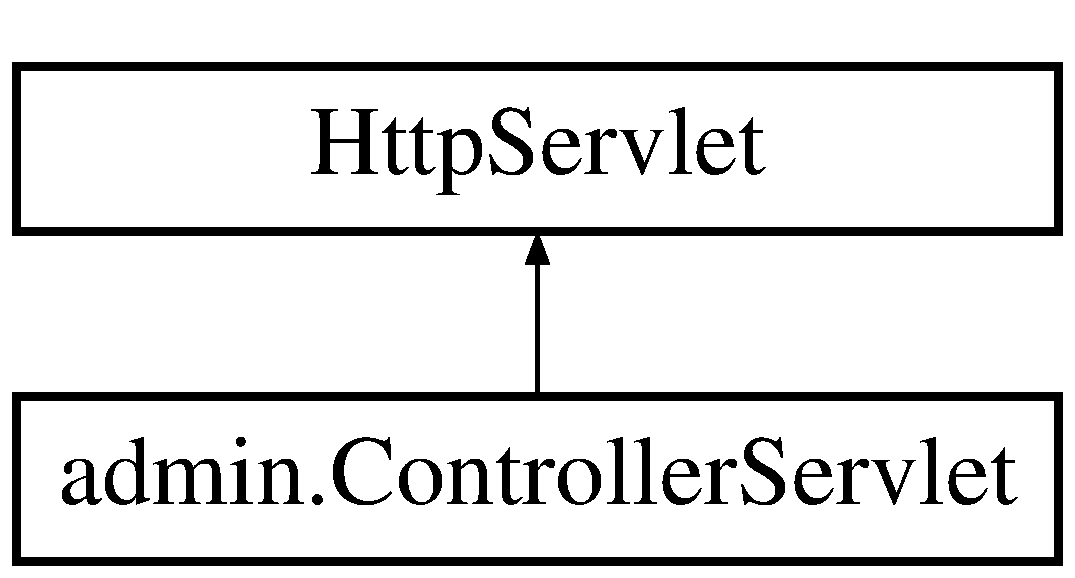
\includegraphics[height=2.000000cm]{classadmin_1_1_controller_servlet}
\end{center}
\end{figure}
\subsection*{Public Member Functions}
\begin{DoxyCompactItemize}
\item 
\hyperlink{classadmin_1_1_controller_servlet_a72f312942007f269cbaf4d86fdd0df36}{Controller\+Servlet} ()
\end{DoxyCompactItemize}
\subsection*{Protected Member Functions}
\begin{DoxyCompactItemize}
\item 
void \hyperlink{classadmin_1_1_controller_servlet_a6b5c24ed500d5a4d110e5cb698187742}{do\+Get} (Http\+Servlet\+Request request, Http\+Servlet\+Response response)  throws Servlet\+Exception, I\+O\+Exception 
\item 
void \hyperlink{classadmin_1_1_controller_servlet_a2c99bb089d8be48e13466b5e5f8c2f95}{do\+Post} (Http\+Servlet\+Request request, Http\+Servlet\+Response response)  throws Servlet\+Exception, I\+O\+Exception 
\end{DoxyCompactItemize}


\subsection{Detailed Description}
Servlet implementation class \hyperlink{classadmin_1_1_controller_servlet}{Controller\+Servlet} 

\subsection{Constructor \& Destructor Documentation}
\index{admin\+::\+Controller\+Servlet@{admin\+::\+Controller\+Servlet}!Controller\+Servlet@{Controller\+Servlet}}
\index{Controller\+Servlet@{Controller\+Servlet}!admin\+::\+Controller\+Servlet@{admin\+::\+Controller\+Servlet}}
\subsubsection[{\texorpdfstring{Controller\+Servlet()}{ControllerServlet()}}]{\setlength{\rightskip}{0pt plus 5cm}admin.\+Controller\+Servlet.\+Controller\+Servlet (
\begin{DoxyParamCaption}
{}
\end{DoxyParamCaption}
)}\hypertarget{classadmin_1_1_controller_servlet_a72f312942007f269cbaf4d86fdd0df36}{}\label{classadmin_1_1_controller_servlet_a72f312942007f269cbaf4d86fdd0df36}
\begin{DoxySeeAlso}{See also}
Http\+Servlet\+::\+Http\+Servlet() 
\end{DoxySeeAlso}


\subsection{Member Function Documentation}
\index{admin\+::\+Controller\+Servlet@{admin\+::\+Controller\+Servlet}!do\+Get@{do\+Get}}
\index{do\+Get@{do\+Get}!admin\+::\+Controller\+Servlet@{admin\+::\+Controller\+Servlet}}
\subsubsection[{\texorpdfstring{do\+Get(\+Http\+Servlet\+Request request, Http\+Servlet\+Response response)}{doGet(HttpServletRequest request, HttpServletResponse response)}}]{\setlength{\rightskip}{0pt plus 5cm}void admin.\+Controller\+Servlet.\+do\+Get (
\begin{DoxyParamCaption}
\item[{Http\+Servlet\+Request}]{request, }
\item[{Http\+Servlet\+Response}]{response}
\end{DoxyParamCaption}
) throws Servlet\+Exception, I\+O\+Exception\hspace{0.3cm}{\ttfamily [protected]}}\hypertarget{classadmin_1_1_controller_servlet_a6b5c24ed500d5a4d110e5cb698187742}{}\label{classadmin_1_1_controller_servlet_a6b5c24ed500d5a4d110e5cb698187742}
\begin{DoxySeeAlso}{See also}
Http\+Servlet\+::do\+Get(\+Http\+Servlet\+Request request, Http\+Servlet\+Response response) 
\end{DoxySeeAlso}
\index{admin\+::\+Controller\+Servlet@{admin\+::\+Controller\+Servlet}!do\+Post@{do\+Post}}
\index{do\+Post@{do\+Post}!admin\+::\+Controller\+Servlet@{admin\+::\+Controller\+Servlet}}
\subsubsection[{\texorpdfstring{do\+Post(\+Http\+Servlet\+Request request, Http\+Servlet\+Response response)}{doPost(HttpServletRequest request, HttpServletResponse response)}}]{\setlength{\rightskip}{0pt plus 5cm}void admin.\+Controller\+Servlet.\+do\+Post (
\begin{DoxyParamCaption}
\item[{Http\+Servlet\+Request}]{request, }
\item[{Http\+Servlet\+Response}]{response}
\end{DoxyParamCaption}
) throws Servlet\+Exception, I\+O\+Exception\hspace{0.3cm}{\ttfamily [protected]}}\hypertarget{classadmin_1_1_controller_servlet_a2c99bb089d8be48e13466b5e5f8c2f95}{}\label{classadmin_1_1_controller_servlet_a2c99bb089d8be48e13466b5e5f8c2f95}
\begin{DoxySeeAlso}{See also}
Http\+Servlet\+::do\+Post(\+Http\+Servlet\+Request request, Http\+Servlet\+Response response) 
\end{DoxySeeAlso}


The documentation for this class was generated from the following file\+:\begin{DoxyCompactItemize}
\item 
Controller\+Servlet.\+java\end{DoxyCompactItemize}

\hypertarget{class_d_bconnect_1_1_d_bconnect}{}\section{D\+Bconnect.\+D\+Bconnect Class Reference}
\label{class_d_bconnect_1_1_d_bconnect}\index{D\+Bconnect.\+D\+Bconnect@{D\+Bconnect.\+D\+Bconnect}}
\subsection*{Public Member Functions}
\begin{DoxyCompactItemize}
\item 
void {\bfseries connect} ()\hypertarget{class_d_bconnect_1_1_d_bconnect_ad65015a1752e59008591e77363cdea85}{}\label{class_d_bconnect_1_1_d_bconnect_ad65015a1752e59008591e77363cdea85}

\item 
Result\+Set {\bfseries query} (String sql)\hypertarget{class_d_bconnect_1_1_d_bconnect_a57b8b689cdd7c5c8847f1217365770be}{}\label{class_d_bconnect_1_1_d_bconnect_a57b8b689cdd7c5c8847f1217365770be}

\item 
int {\bfseries update} (String sql)\hypertarget{class_d_bconnect_1_1_d_bconnect_a3649fbeed1ca73503f4c4fe64ec6224f}{}\label{class_d_bconnect_1_1_d_bconnect_a3649fbeed1ca73503f4c4fe64ec6224f}

\item 
void {\bfseries close} ()\hypertarget{class_d_bconnect_1_1_d_bconnect_a6036d909edae5c3d94b39e336d0a876e}{}\label{class_d_bconnect_1_1_d_bconnect_a6036d909edae5c3d94b39e336d0a876e}

\end{DoxyCompactItemize}
\subsection*{Static Public Member Functions}
\begin{DoxyCompactItemize}
\item 
static void {\bfseries main} (String\mbox{[}$\,$\mbox{]} args)\hypertarget{class_d_bconnect_1_1_d_bconnect_aad4e1274e0184b62c3e1c3dca1cf3563}{}\label{class_d_bconnect_1_1_d_bconnect_aad4e1274e0184b62c3e1c3dca1cf3563}

\end{DoxyCompactItemize}
\subsection*{Static Public Attributes}
\begin{DoxyCompactItemize}
\item 
static Result\+Set {\bfseries res} = null\hypertarget{class_d_bconnect_1_1_d_bconnect_af39df1d2d107724daeceb6c8585f521a}{}\label{class_d_bconnect_1_1_d_bconnect_af39df1d2d107724daeceb6c8585f521a}

\end{DoxyCompactItemize}


The documentation for this class was generated from the following file\+:\begin{DoxyCompactItemize}
\item 
D\+Bconnect.\+java\end{DoxyCompactItemize}

\hypertarget{classhistory_1_1_history_bean}{}\section{history.\+History\+Bean Class Reference}
\label{classhistory_1_1_history_bean}\index{history.\+History\+Bean@{history.\+History\+Bean}}
\subsection*{Public Member Functions}
\begin{DoxyCompactItemize}
\item 
boolean {\bfseries is\+Loaded} ()\hypertarget{classhistory_1_1_history_bean_ad8f46a0ae1fb61150f32009ce9883693}{}\label{classhistory_1_1_history_bean_ad8f46a0ae1fb61150f32009ce9883693}

\item 
int {\bfseries get\+Row\+Num} ()\hypertarget{classhistory_1_1_history_bean_a9d05f9cc6dad82412af5888c9e694a12}{}\label{classhistory_1_1_history_bean_a9d05f9cc6dad82412af5888c9e694a12}

\item 
String\mbox{[}$\,$\mbox{]}\mbox{[}$\,$\mbox{]} {\bfseries get\+Book\+Info} ()\hypertarget{classhistory_1_1_history_bean_ae66608c4f577b70115f257f75551098f}{}\label{classhistory_1_1_history_bean_ae66608c4f577b70115f257f75551098f}

\item 
void {\bfseries set\+User\+ID} (String id)\hypertarget{classhistory_1_1_history_bean_aa599d648e48b45d460b0e64e84c6bb3a}{}\label{classhistory_1_1_history_bean_aa599d648e48b45d460b0e64e84c6bb3a}

\item 
void {\bfseries set\+Book\+Info} (String id)\hypertarget{classhistory_1_1_history_bean_a8c40038ea495990a54d7f3bcfae304d7}{}\label{classhistory_1_1_history_bean_a8c40038ea495990a54d7f3bcfae304d7}

\end{DoxyCompactItemize}
\subsection*{Static Public Member Functions}
\begin{DoxyCompactItemize}
\item 
static void {\bfseries clear} ()\hypertarget{classhistory_1_1_history_bean_a4028b20aae7962ee093b38c5b3e4517a}{}\label{classhistory_1_1_history_bean_a4028b20aae7962ee093b38c5b3e4517a}

\item 
static void {\bfseries main} (String\mbox{[}$\,$\mbox{]} args)\hypertarget{classhistory_1_1_history_bean_ac709fce9384d1ee0e1352383e5531f4d}{}\label{classhistory_1_1_history_bean_ac709fce9384d1ee0e1352383e5531f4d}

\end{DoxyCompactItemize}


The documentation for this class was generated from the following file\+:\begin{DoxyCompactItemize}
\item 
History\+Bean.\+java\end{DoxyCompactItemize}

\hypertarget{classloan_1_1_loan_bean}{}\section{loan.\+Loan\+Bean Class Reference}
\label{classloan_1_1_loan_bean}\index{loan.\+Loan\+Bean@{loan.\+Loan\+Bean}}
\subsection*{Public Member Functions}
\begin{DoxyCompactItemize}
\item 
boolean {\bfseries is\+Loaded} ()\hypertarget{classloan_1_1_loan_bean_af8b0094d96ab6a310c078fcc93f5de50}{}\label{classloan_1_1_loan_bean_af8b0094d96ab6a310c078fcc93f5de50}

\item 
int {\bfseries get\+Row\+Num} ()\hypertarget{classloan_1_1_loan_bean_a877dd9a33be3fb24db21e31977e4330c}{}\label{classloan_1_1_loan_bean_a877dd9a33be3fb24db21e31977e4330c}

\item 
String\mbox{[}$\,$\mbox{]}\mbox{[}$\,$\mbox{]} {\bfseries get\+Book\+Info} ()\hypertarget{classloan_1_1_loan_bean_ac59567271b218b8a6a59eb7723964f64}{}\label{classloan_1_1_loan_bean_ac59567271b218b8a6a59eb7723964f64}

\item 
void {\bfseries set\+User\+ID} (String id)\hypertarget{classloan_1_1_loan_bean_a38f9f0a750e55cd377d34f5b9c4a9c0b}{}\label{classloan_1_1_loan_bean_a38f9f0a750e55cd377d34f5b9c4a9c0b}

\item 
void {\bfseries set\+Book\+Info} (String id)\hypertarget{classloan_1_1_loan_bean_a7c80ca228be4bd4438e4a4bef40dc0d0}{}\label{classloan_1_1_loan_bean_a7c80ca228be4bd4438e4a4bef40dc0d0}

\end{DoxyCompactItemize}
\subsection*{Static Public Member Functions}
\begin{DoxyCompactItemize}
\item 
static void {\bfseries clear} ()\hypertarget{classloan_1_1_loan_bean_ac5f11c145a3b4a73c97f82bdc3beb07d}{}\label{classloan_1_1_loan_bean_ac5f11c145a3b4a73c97f82bdc3beb07d}

\item 
static void {\bfseries main} (String\mbox{[}$\,$\mbox{]} args)\hypertarget{classloan_1_1_loan_bean_a7c98ca3abd92ebc7dde7117c1b9471d7}{}\label{classloan_1_1_loan_bean_a7c98ca3abd92ebc7dde7117c1b9471d7}

\end{DoxyCompactItemize}


The documentation for this class was generated from the following file\+:\begin{DoxyCompactItemize}
\item 
Loan\+Bean.\+java\end{DoxyCompactItemize}

\hypertarget{classlogin_1_1_login_servlet}{}\section{login.\+Login\+Servlet Class Reference}
\label{classlogin_1_1_login_servlet}\index{login.\+Login\+Servlet@{login.\+Login\+Servlet}}
Inheritance diagram for login.\+Login\+Servlet\+:\begin{figure}[H]
\begin{center}
\leavevmode
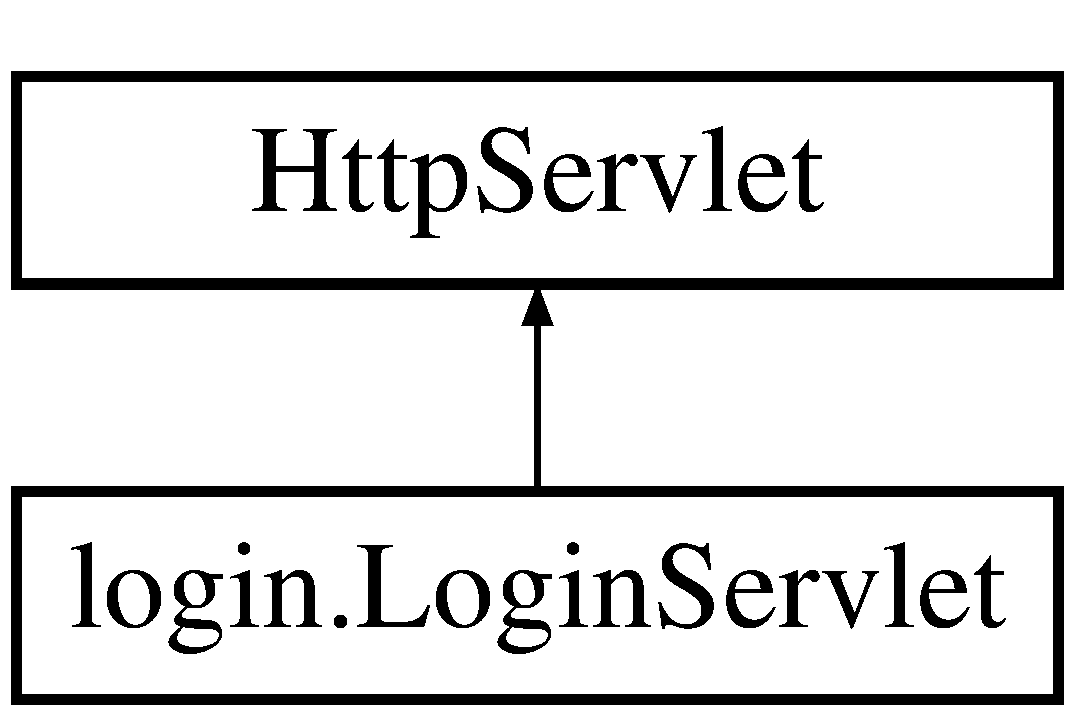
\includegraphics[height=2.000000cm]{classlogin_1_1_login_servlet}
\end{center}
\end{figure}
\subsection*{Public Member Functions}
\begin{DoxyCompactItemize}
\item 
\hyperlink{classlogin_1_1_login_servlet_af8c37b0240335c1641b25c63522a974d}{Login\+Servlet} ()
\end{DoxyCompactItemize}
\subsection*{Protected Member Functions}
\begin{DoxyCompactItemize}
\item 
void \hyperlink{classlogin_1_1_login_servlet_a983f5828fbf3bb2e11488db56fd2e4e2}{do\+Get} (Http\+Servlet\+Request request, Http\+Servlet\+Response response)  throws Servlet\+Exception, I\+O\+Exception 
\item 
void \hyperlink{classlogin_1_1_login_servlet_a64cfb5af5fdfe51e081b7004a54b1404}{do\+Post} (Http\+Servlet\+Request request, Http\+Servlet\+Response response)  throws Servlet\+Exception, I\+O\+Exception 
\end{DoxyCompactItemize}


\subsection{Detailed Description}
Servlet implementation class \hyperlink{classlogin_1_1_login_servlet}{Login\+Servlet} 

\subsection{Constructor \& Destructor Documentation}
\index{login\+::\+Login\+Servlet@{login\+::\+Login\+Servlet}!Login\+Servlet@{Login\+Servlet}}
\index{Login\+Servlet@{Login\+Servlet}!login\+::\+Login\+Servlet@{login\+::\+Login\+Servlet}}
\subsubsection[{\texorpdfstring{Login\+Servlet()}{LoginServlet()}}]{\setlength{\rightskip}{0pt plus 5cm}login.\+Login\+Servlet.\+Login\+Servlet (
\begin{DoxyParamCaption}
{}
\end{DoxyParamCaption}
)}\hypertarget{classlogin_1_1_login_servlet_af8c37b0240335c1641b25c63522a974d}{}\label{classlogin_1_1_login_servlet_af8c37b0240335c1641b25c63522a974d}
\begin{DoxySeeAlso}{See also}
Http\+Servlet\+::\+Http\+Servlet() 
\end{DoxySeeAlso}


\subsection{Member Function Documentation}
\index{login\+::\+Login\+Servlet@{login\+::\+Login\+Servlet}!do\+Get@{do\+Get}}
\index{do\+Get@{do\+Get}!login\+::\+Login\+Servlet@{login\+::\+Login\+Servlet}}
\subsubsection[{\texorpdfstring{do\+Get(\+Http\+Servlet\+Request request, Http\+Servlet\+Response response)}{doGet(HttpServletRequest request, HttpServletResponse response)}}]{\setlength{\rightskip}{0pt plus 5cm}void login.\+Login\+Servlet.\+do\+Get (
\begin{DoxyParamCaption}
\item[{Http\+Servlet\+Request}]{request, }
\item[{Http\+Servlet\+Response}]{response}
\end{DoxyParamCaption}
) throws Servlet\+Exception, I\+O\+Exception\hspace{0.3cm}{\ttfamily [protected]}}\hypertarget{classlogin_1_1_login_servlet_a983f5828fbf3bb2e11488db56fd2e4e2}{}\label{classlogin_1_1_login_servlet_a983f5828fbf3bb2e11488db56fd2e4e2}
\begin{DoxySeeAlso}{See also}
Http\+Servlet\+::do\+Get(\+Http\+Servlet\+Request request, Http\+Servlet\+Response response) 
\end{DoxySeeAlso}
\index{login\+::\+Login\+Servlet@{login\+::\+Login\+Servlet}!do\+Post@{do\+Post}}
\index{do\+Post@{do\+Post}!login\+::\+Login\+Servlet@{login\+::\+Login\+Servlet}}
\subsubsection[{\texorpdfstring{do\+Post(\+Http\+Servlet\+Request request, Http\+Servlet\+Response response)}{doPost(HttpServletRequest request, HttpServletResponse response)}}]{\setlength{\rightskip}{0pt plus 5cm}void login.\+Login\+Servlet.\+do\+Post (
\begin{DoxyParamCaption}
\item[{Http\+Servlet\+Request}]{request, }
\item[{Http\+Servlet\+Response}]{response}
\end{DoxyParamCaption}
) throws Servlet\+Exception, I\+O\+Exception\hspace{0.3cm}{\ttfamily [protected]}}\hypertarget{classlogin_1_1_login_servlet_a64cfb5af5fdfe51e081b7004a54b1404}{}\label{classlogin_1_1_login_servlet_a64cfb5af5fdfe51e081b7004a54b1404}
\begin{DoxySeeAlso}{See also}
Http\+Servlet\+::do\+Post(\+Http\+Servlet\+Request request, Http\+Servlet\+Response response) 
\end{DoxySeeAlso}


The documentation for this class was generated from the following file\+:\begin{DoxyCompactItemize}
\item 
Login\+Servlet.\+java\end{DoxyCompactItemize}

\hypertarget{classadmin_1_1_modify_bean}{}\section{admin.\+Modify\+Bean Class Reference}
\label{classadmin_1_1_modify_bean}\index{admin.\+Modify\+Bean@{admin.\+Modify\+Bean}}
\subsection*{Public Member Functions}
\begin{DoxyCompactItemize}
\item 
boolean {\bfseries is\+Load} ()\hypertarget{classadmin_1_1_modify_bean_a504e0ce1bcef8665104cd2c7f2a92a90}{}\label{classadmin_1_1_modify_bean_a504e0ce1bcef8665104cd2c7f2a92a90}

\item 
void {\bfseries set} (String id)\hypertarget{classadmin_1_1_modify_bean_a2452b17b38f39a9cfd782c30979024b5}{}\label{classadmin_1_1_modify_bean_a2452b17b38f39a9cfd782c30979024b5}

\item 
String {\bfseries get\+ID} ()\hypertarget{classadmin_1_1_modify_bean_a1edb15b8795b61fb1c3869473dc4fd65}{}\label{classadmin_1_1_modify_bean_a1edb15b8795b61fb1c3869473dc4fd65}

\item 
void {\bfseries load\+Book\+Info} ()\hypertarget{classadmin_1_1_modify_bean_a0854744826c47dc16b1d49d0f9b02e59}{}\label{classadmin_1_1_modify_bean_a0854744826c47dc16b1d49d0f9b02e59}

\item 
String {\bfseries get\+Book\+Info} (String info)\hypertarget{classadmin_1_1_modify_bean_aef1625745802811d0d717bddcf79a858}{}\label{classadmin_1_1_modify_bean_aef1625745802811d0d717bddcf79a858}

\end{DoxyCompactItemize}
\subsection*{Static Public Member Functions}
\begin{DoxyCompactItemize}
\item 
static void {\bfseries main} (String\mbox{[}$\,$\mbox{]} args)\hypertarget{classadmin_1_1_modify_bean_a9966a4574bc56a7b121596ec3a8e1400}{}\label{classadmin_1_1_modify_bean_a9966a4574bc56a7b121596ec3a8e1400}

\end{DoxyCompactItemize}


The documentation for this class was generated from the following file\+:\begin{DoxyCompactItemize}
\item 
Modify\+Bean.\+java\end{DoxyCompactItemize}

\hypertarget{classadmin_1_1_modify_servlet}{}\section{admin.\+Modify\+Servlet Class Reference}
\label{classadmin_1_1_modify_servlet}\index{admin.\+Modify\+Servlet@{admin.\+Modify\+Servlet}}
Inheritance diagram for admin.\+Modify\+Servlet\+:\begin{figure}[H]
\begin{center}
\leavevmode
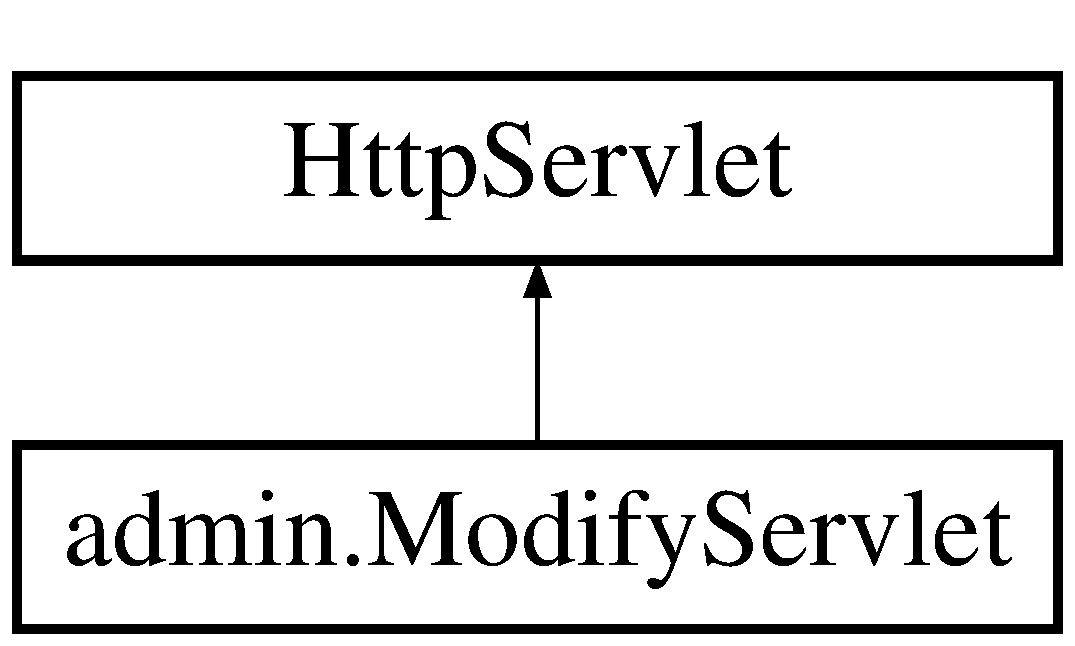
\includegraphics[height=2.000000cm]{classadmin_1_1_modify_servlet}
\end{center}
\end{figure}
\subsection*{Public Member Functions}
\begin{DoxyCompactItemize}
\item 
\hyperlink{classadmin_1_1_modify_servlet_a8afe56ea4faeb9511cdf1ad20497e3bc}{Modify\+Servlet} ()
\end{DoxyCompactItemize}
\subsection*{Protected Member Functions}
\begin{DoxyCompactItemize}
\item 
void \hyperlink{classadmin_1_1_modify_servlet_a58774982d5e6398cb6d3016f1b652c22}{do\+Get} (Http\+Servlet\+Request request, Http\+Servlet\+Response response)  throws Servlet\+Exception, I\+O\+Exception 
\item 
void \hyperlink{classadmin_1_1_modify_servlet_a84c3c7bb3f9338a98c39c19557847422}{do\+Post} (Http\+Servlet\+Request request, Http\+Servlet\+Response response)  throws Servlet\+Exception, I\+O\+Exception 
\end{DoxyCompactItemize}


\subsection{Detailed Description}
Servlet implementation class \hyperlink{classadmin_1_1_modify_servlet}{Modify\+Servlet} 

\subsection{Constructor \& Destructor Documentation}
\index{admin\+::\+Modify\+Servlet@{admin\+::\+Modify\+Servlet}!Modify\+Servlet@{Modify\+Servlet}}
\index{Modify\+Servlet@{Modify\+Servlet}!admin\+::\+Modify\+Servlet@{admin\+::\+Modify\+Servlet}}
\subsubsection[{\texorpdfstring{Modify\+Servlet()}{ModifyServlet()}}]{\setlength{\rightskip}{0pt plus 5cm}admin.\+Modify\+Servlet.\+Modify\+Servlet (
\begin{DoxyParamCaption}
{}
\end{DoxyParamCaption}
)}\hypertarget{classadmin_1_1_modify_servlet_a8afe56ea4faeb9511cdf1ad20497e3bc}{}\label{classadmin_1_1_modify_servlet_a8afe56ea4faeb9511cdf1ad20497e3bc}
\begin{DoxySeeAlso}{See also}
Http\+Servlet\+::\+Http\+Servlet() 
\end{DoxySeeAlso}


\subsection{Member Function Documentation}
\index{admin\+::\+Modify\+Servlet@{admin\+::\+Modify\+Servlet}!do\+Get@{do\+Get}}
\index{do\+Get@{do\+Get}!admin\+::\+Modify\+Servlet@{admin\+::\+Modify\+Servlet}}
\subsubsection[{\texorpdfstring{do\+Get(\+Http\+Servlet\+Request request, Http\+Servlet\+Response response)}{doGet(HttpServletRequest request, HttpServletResponse response)}}]{\setlength{\rightskip}{0pt plus 5cm}void admin.\+Modify\+Servlet.\+do\+Get (
\begin{DoxyParamCaption}
\item[{Http\+Servlet\+Request}]{request, }
\item[{Http\+Servlet\+Response}]{response}
\end{DoxyParamCaption}
) throws Servlet\+Exception, I\+O\+Exception\hspace{0.3cm}{\ttfamily [protected]}}\hypertarget{classadmin_1_1_modify_servlet_a58774982d5e6398cb6d3016f1b652c22}{}\label{classadmin_1_1_modify_servlet_a58774982d5e6398cb6d3016f1b652c22}
\begin{DoxySeeAlso}{See also}
Http\+Servlet\+::do\+Get(\+Http\+Servlet\+Request request, Http\+Servlet\+Response response) 
\end{DoxySeeAlso}
\index{admin\+::\+Modify\+Servlet@{admin\+::\+Modify\+Servlet}!do\+Post@{do\+Post}}
\index{do\+Post@{do\+Post}!admin\+::\+Modify\+Servlet@{admin\+::\+Modify\+Servlet}}
\subsubsection[{\texorpdfstring{do\+Post(\+Http\+Servlet\+Request request, Http\+Servlet\+Response response)}{doPost(HttpServletRequest request, HttpServletResponse response)}}]{\setlength{\rightskip}{0pt plus 5cm}void admin.\+Modify\+Servlet.\+do\+Post (
\begin{DoxyParamCaption}
\item[{Http\+Servlet\+Request}]{request, }
\item[{Http\+Servlet\+Response}]{response}
\end{DoxyParamCaption}
) throws Servlet\+Exception, I\+O\+Exception\hspace{0.3cm}{\ttfamily [protected]}}\hypertarget{classadmin_1_1_modify_servlet_a84c3c7bb3f9338a98c39c19557847422}{}\label{classadmin_1_1_modify_servlet_a84c3c7bb3f9338a98c39c19557847422}
\begin{DoxySeeAlso}{See also}
Http\+Servlet\+::do\+Post(\+Http\+Servlet\+Request request, Http\+Servlet\+Response response) 
\end{DoxySeeAlso}


The documentation for this class was generated from the following file\+:\begin{DoxyCompactItemize}
\item 
Modify\+Servlet.\+java\end{DoxyCompactItemize}

\hypertarget{classadvanced_1_1_recommend_servlet}{}\section{advanced.\+Recommend\+Servlet Class Reference}
\label{classadvanced_1_1_recommend_servlet}\index{advanced.\+Recommend\+Servlet@{advanced.\+Recommend\+Servlet}}
Inheritance diagram for advanced.\+Recommend\+Servlet\+:\begin{figure}[H]
\begin{center}
\leavevmode
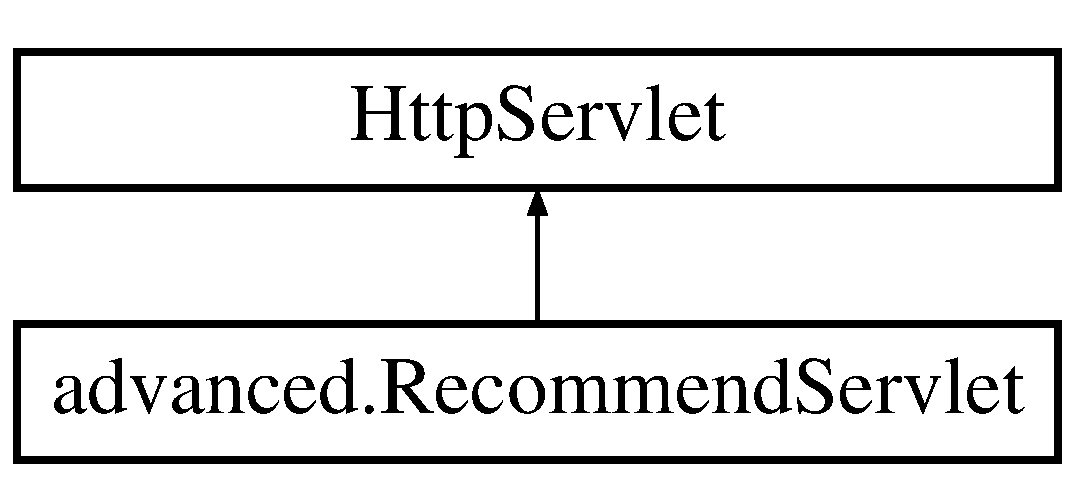
\includegraphics[height=2.000000cm]{classadvanced_1_1_recommend_servlet}
\end{center}
\end{figure}
\subsection*{Public Member Functions}
\begin{DoxyCompactItemize}
\item 
\hyperlink{classadvanced_1_1_recommend_servlet_a0b65a3f29a28d30346b9478aab2fccb6}{Recommend\+Servlet} ()
\end{DoxyCompactItemize}
\subsection*{Protected Member Functions}
\begin{DoxyCompactItemize}
\item 
void \hyperlink{classadvanced_1_1_recommend_servlet_a053694ba555f8bad9dbb25f3f93326fc}{do\+Get} (Http\+Servlet\+Request request, Http\+Servlet\+Response response)  throws Servlet\+Exception, I\+O\+Exception 
\item 
void \hyperlink{classadvanced_1_1_recommend_servlet_af15682cbfbf5f21594538f20d8a8f450}{do\+Post} (Http\+Servlet\+Request request, Http\+Servlet\+Response response)  throws Servlet\+Exception, I\+O\+Exception 
\end{DoxyCompactItemize}


\subsection{Detailed Description}
Servlet implementation class \hyperlink{classadvanced_1_1_recommend_servlet}{Recommend\+Servlet} 

\subsection{Constructor \& Destructor Documentation}
\index{advanced\+::\+Recommend\+Servlet@{advanced\+::\+Recommend\+Servlet}!Recommend\+Servlet@{Recommend\+Servlet}}
\index{Recommend\+Servlet@{Recommend\+Servlet}!advanced\+::\+Recommend\+Servlet@{advanced\+::\+Recommend\+Servlet}}
\subsubsection[{\texorpdfstring{Recommend\+Servlet()}{RecommendServlet()}}]{\setlength{\rightskip}{0pt plus 5cm}advanced.\+Recommend\+Servlet.\+Recommend\+Servlet (
\begin{DoxyParamCaption}
{}
\end{DoxyParamCaption}
)}\hypertarget{classadvanced_1_1_recommend_servlet_a0b65a3f29a28d30346b9478aab2fccb6}{}\label{classadvanced_1_1_recommend_servlet_a0b65a3f29a28d30346b9478aab2fccb6}
\begin{DoxySeeAlso}{See also}
Http\+Servlet\+::\+Http\+Servlet() 
\end{DoxySeeAlso}


\subsection{Member Function Documentation}
\index{advanced\+::\+Recommend\+Servlet@{advanced\+::\+Recommend\+Servlet}!do\+Get@{do\+Get}}
\index{do\+Get@{do\+Get}!advanced\+::\+Recommend\+Servlet@{advanced\+::\+Recommend\+Servlet}}
\subsubsection[{\texorpdfstring{do\+Get(\+Http\+Servlet\+Request request, Http\+Servlet\+Response response)}{doGet(HttpServletRequest request, HttpServletResponse response)}}]{\setlength{\rightskip}{0pt plus 5cm}void advanced.\+Recommend\+Servlet.\+do\+Get (
\begin{DoxyParamCaption}
\item[{Http\+Servlet\+Request}]{request, }
\item[{Http\+Servlet\+Response}]{response}
\end{DoxyParamCaption}
) throws Servlet\+Exception, I\+O\+Exception\hspace{0.3cm}{\ttfamily [protected]}}\hypertarget{classadvanced_1_1_recommend_servlet_a053694ba555f8bad9dbb25f3f93326fc}{}\label{classadvanced_1_1_recommend_servlet_a053694ba555f8bad9dbb25f3f93326fc}
\begin{DoxySeeAlso}{See also}
Http\+Servlet\+::do\+Get(\+Http\+Servlet\+Request request, Http\+Servlet\+Response response) 
\end{DoxySeeAlso}
\index{advanced\+::\+Recommend\+Servlet@{advanced\+::\+Recommend\+Servlet}!do\+Post@{do\+Post}}
\index{do\+Post@{do\+Post}!advanced\+::\+Recommend\+Servlet@{advanced\+::\+Recommend\+Servlet}}
\subsubsection[{\texorpdfstring{do\+Post(\+Http\+Servlet\+Request request, Http\+Servlet\+Response response)}{doPost(HttpServletRequest request, HttpServletResponse response)}}]{\setlength{\rightskip}{0pt plus 5cm}void advanced.\+Recommend\+Servlet.\+do\+Post (
\begin{DoxyParamCaption}
\item[{Http\+Servlet\+Request}]{request, }
\item[{Http\+Servlet\+Response}]{response}
\end{DoxyParamCaption}
) throws Servlet\+Exception, I\+O\+Exception\hspace{0.3cm}{\ttfamily [protected]}}\hypertarget{classadvanced_1_1_recommend_servlet_af15682cbfbf5f21594538f20d8a8f450}{}\label{classadvanced_1_1_recommend_servlet_af15682cbfbf5f21594538f20d8a8f450}
\begin{DoxySeeAlso}{See also}
Http\+Servlet\+::do\+Post(\+Http\+Servlet\+Request request, Http\+Servlet\+Response response) 
\end{DoxySeeAlso}


The documentation for this class was generated from the following file\+:\begin{DoxyCompactItemize}
\item 
Recommend\+Servlet.\+java\end{DoxyCompactItemize}

\hypertarget{classadmin_1_1_remove_servlet}{}\section{admin.\+Remove\+Servlet Class Reference}
\label{classadmin_1_1_remove_servlet}\index{admin.\+Remove\+Servlet@{admin.\+Remove\+Servlet}}
Inheritance diagram for admin.\+Remove\+Servlet\+:\begin{figure}[H]
\begin{center}
\leavevmode
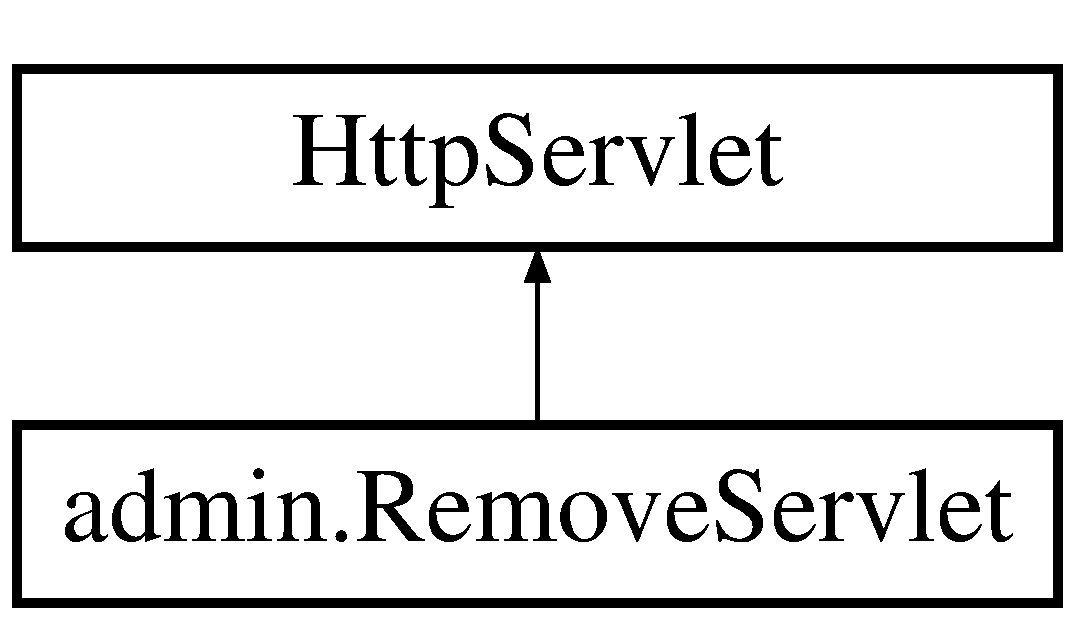
\includegraphics[height=2.000000cm]{classadmin_1_1_remove_servlet}
\end{center}
\end{figure}
\subsection*{Public Member Functions}
\begin{DoxyCompactItemize}
\item 
\hyperlink{classadmin_1_1_remove_servlet_a4a37e587d1e6d20307aec984fbccb9e5}{Remove\+Servlet} ()
\end{DoxyCompactItemize}
\subsection*{Protected Member Functions}
\begin{DoxyCompactItemize}
\item 
void \hyperlink{classadmin_1_1_remove_servlet_abeaea85014c5e6cb6eded135ebb1cdec}{do\+Get} (Http\+Servlet\+Request request, Http\+Servlet\+Response response)  throws Servlet\+Exception, I\+O\+Exception 
\item 
void \hyperlink{classadmin_1_1_remove_servlet_a9d4e3b4e08640f72088a481aeb264c9a}{do\+Post} (Http\+Servlet\+Request request, Http\+Servlet\+Response response)  throws Servlet\+Exception, I\+O\+Exception 
\end{DoxyCompactItemize}


\subsection{Detailed Description}
Servlet implementation class \hyperlink{classadmin_1_1_remove_servlet}{Remove\+Servlet} 

\subsection{Constructor \& Destructor Documentation}
\index{admin\+::\+Remove\+Servlet@{admin\+::\+Remove\+Servlet}!Remove\+Servlet@{Remove\+Servlet}}
\index{Remove\+Servlet@{Remove\+Servlet}!admin\+::\+Remove\+Servlet@{admin\+::\+Remove\+Servlet}}
\subsubsection[{\texorpdfstring{Remove\+Servlet()}{RemoveServlet()}}]{\setlength{\rightskip}{0pt plus 5cm}admin.\+Remove\+Servlet.\+Remove\+Servlet (
\begin{DoxyParamCaption}
{}
\end{DoxyParamCaption}
)}\hypertarget{classadmin_1_1_remove_servlet_a4a37e587d1e6d20307aec984fbccb9e5}{}\label{classadmin_1_1_remove_servlet_a4a37e587d1e6d20307aec984fbccb9e5}
\begin{DoxySeeAlso}{See also}
Http\+Servlet\+::\+Http\+Servlet() 
\end{DoxySeeAlso}


\subsection{Member Function Documentation}
\index{admin\+::\+Remove\+Servlet@{admin\+::\+Remove\+Servlet}!do\+Get@{do\+Get}}
\index{do\+Get@{do\+Get}!admin\+::\+Remove\+Servlet@{admin\+::\+Remove\+Servlet}}
\subsubsection[{\texorpdfstring{do\+Get(\+Http\+Servlet\+Request request, Http\+Servlet\+Response response)}{doGet(HttpServletRequest request, HttpServletResponse response)}}]{\setlength{\rightskip}{0pt plus 5cm}void admin.\+Remove\+Servlet.\+do\+Get (
\begin{DoxyParamCaption}
\item[{Http\+Servlet\+Request}]{request, }
\item[{Http\+Servlet\+Response}]{response}
\end{DoxyParamCaption}
) throws Servlet\+Exception, I\+O\+Exception\hspace{0.3cm}{\ttfamily [protected]}}\hypertarget{classadmin_1_1_remove_servlet_abeaea85014c5e6cb6eded135ebb1cdec}{}\label{classadmin_1_1_remove_servlet_abeaea85014c5e6cb6eded135ebb1cdec}
\begin{DoxySeeAlso}{See also}
Http\+Servlet\+::do\+Get(\+Http\+Servlet\+Request request, Http\+Servlet\+Response response) 
\end{DoxySeeAlso}
\index{admin\+::\+Remove\+Servlet@{admin\+::\+Remove\+Servlet}!do\+Post@{do\+Post}}
\index{do\+Post@{do\+Post}!admin\+::\+Remove\+Servlet@{admin\+::\+Remove\+Servlet}}
\subsubsection[{\texorpdfstring{do\+Post(\+Http\+Servlet\+Request request, Http\+Servlet\+Response response)}{doPost(HttpServletRequest request, HttpServletResponse response)}}]{\setlength{\rightskip}{0pt plus 5cm}void admin.\+Remove\+Servlet.\+do\+Post (
\begin{DoxyParamCaption}
\item[{Http\+Servlet\+Request}]{request, }
\item[{Http\+Servlet\+Response}]{response}
\end{DoxyParamCaption}
) throws Servlet\+Exception, I\+O\+Exception\hspace{0.3cm}{\ttfamily [protected]}}\hypertarget{classadmin_1_1_remove_servlet_a9d4e3b4e08640f72088a481aeb264c9a}{}\label{classadmin_1_1_remove_servlet_a9d4e3b4e08640f72088a481aeb264c9a}
\begin{DoxySeeAlso}{See also}
Http\+Servlet\+::do\+Post(\+Http\+Servlet\+Request request, Http\+Servlet\+Response response) 
\end{DoxySeeAlso}


The documentation for this class was generated from the following file\+:\begin{DoxyCompactItemize}
\item 
Remove\+Servlet.\+java\end{DoxyCompactItemize}

\hypertarget{classadvanced_1_1_request_servlet}{}\section{advanced.\+Request\+Servlet Class Reference}
\label{classadvanced_1_1_request_servlet}\index{advanced.\+Request\+Servlet@{advanced.\+Request\+Servlet}}
Inheritance diagram for advanced.\+Request\+Servlet\+:\begin{figure}[H]
\begin{center}
\leavevmode
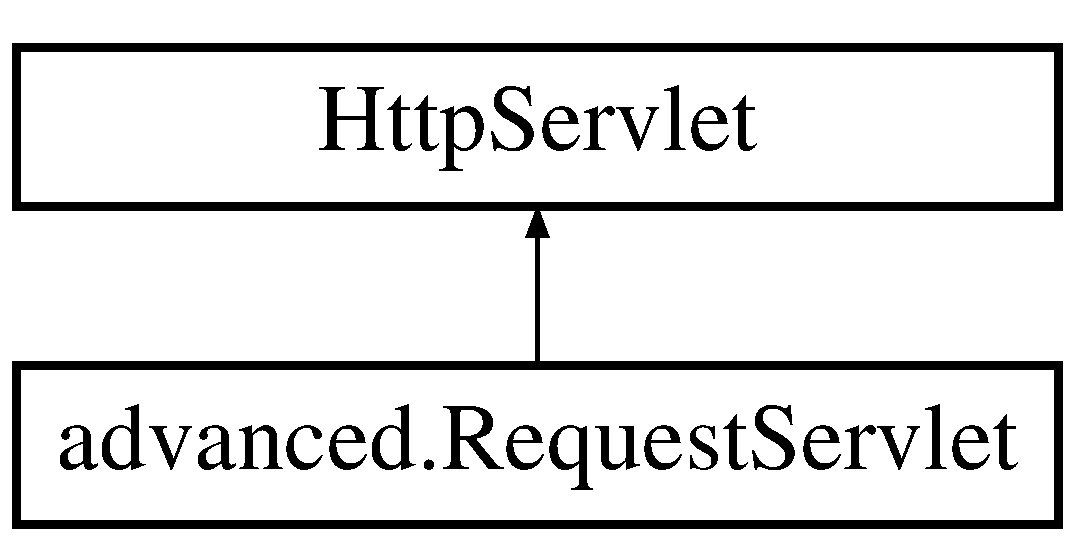
\includegraphics[height=2.000000cm]{classadvanced_1_1_request_servlet}
\end{center}
\end{figure}
\subsection*{Public Member Functions}
\begin{DoxyCompactItemize}
\item 
\hyperlink{classadvanced_1_1_request_servlet_ac03b771e0d06eb69766ac2df52cb5f2f}{Request\+Servlet} ()
\end{DoxyCompactItemize}
\subsection*{Protected Member Functions}
\begin{DoxyCompactItemize}
\item 
void \hyperlink{classadvanced_1_1_request_servlet_a56fd652c4380a401d80754ca12cdbbbc}{do\+Get} (Http\+Servlet\+Request request, Http\+Servlet\+Response response)  throws Servlet\+Exception, I\+O\+Exception 
\item 
void \hyperlink{classadvanced_1_1_request_servlet_acd5fa3621347affb7135a9a44853265f}{do\+Post} (Http\+Servlet\+Request request, Http\+Servlet\+Response response)  throws Servlet\+Exception, I\+O\+Exception 
\end{DoxyCompactItemize}


\subsection{Detailed Description}
Servlet implementation class \hyperlink{classadvanced_1_1_request_servlet}{Request\+Servlet} 

\subsection{Constructor \& Destructor Documentation}
\index{advanced\+::\+Request\+Servlet@{advanced\+::\+Request\+Servlet}!Request\+Servlet@{Request\+Servlet}}
\index{Request\+Servlet@{Request\+Servlet}!advanced\+::\+Request\+Servlet@{advanced\+::\+Request\+Servlet}}
\subsubsection[{\texorpdfstring{Request\+Servlet()}{RequestServlet()}}]{\setlength{\rightskip}{0pt plus 5cm}advanced.\+Request\+Servlet.\+Request\+Servlet (
\begin{DoxyParamCaption}
{}
\end{DoxyParamCaption}
)}\hypertarget{classadvanced_1_1_request_servlet_ac03b771e0d06eb69766ac2df52cb5f2f}{}\label{classadvanced_1_1_request_servlet_ac03b771e0d06eb69766ac2df52cb5f2f}
\begin{DoxySeeAlso}{See also}
Http\+Servlet\+::\+Http\+Servlet() 
\end{DoxySeeAlso}


\subsection{Member Function Documentation}
\index{advanced\+::\+Request\+Servlet@{advanced\+::\+Request\+Servlet}!do\+Get@{do\+Get}}
\index{do\+Get@{do\+Get}!advanced\+::\+Request\+Servlet@{advanced\+::\+Request\+Servlet}}
\subsubsection[{\texorpdfstring{do\+Get(\+Http\+Servlet\+Request request, Http\+Servlet\+Response response)}{doGet(HttpServletRequest request, HttpServletResponse response)}}]{\setlength{\rightskip}{0pt plus 5cm}void advanced.\+Request\+Servlet.\+do\+Get (
\begin{DoxyParamCaption}
\item[{Http\+Servlet\+Request}]{request, }
\item[{Http\+Servlet\+Response}]{response}
\end{DoxyParamCaption}
) throws Servlet\+Exception, I\+O\+Exception\hspace{0.3cm}{\ttfamily [protected]}}\hypertarget{classadvanced_1_1_request_servlet_a56fd652c4380a401d80754ca12cdbbbc}{}\label{classadvanced_1_1_request_servlet_a56fd652c4380a401d80754ca12cdbbbc}
\begin{DoxySeeAlso}{See also}
Http\+Servlet\+::do\+Get(\+Http\+Servlet\+Request request, Http\+Servlet\+Response response) 
\end{DoxySeeAlso}
\index{advanced\+::\+Request\+Servlet@{advanced\+::\+Request\+Servlet}!do\+Post@{do\+Post}}
\index{do\+Post@{do\+Post}!advanced\+::\+Request\+Servlet@{advanced\+::\+Request\+Servlet}}
\subsubsection[{\texorpdfstring{do\+Post(\+Http\+Servlet\+Request request, Http\+Servlet\+Response response)}{doPost(HttpServletRequest request, HttpServletResponse response)}}]{\setlength{\rightskip}{0pt plus 5cm}void advanced.\+Request\+Servlet.\+do\+Post (
\begin{DoxyParamCaption}
\item[{Http\+Servlet\+Request}]{request, }
\item[{Http\+Servlet\+Response}]{response}
\end{DoxyParamCaption}
) throws Servlet\+Exception, I\+O\+Exception\hspace{0.3cm}{\ttfamily [protected]}}\hypertarget{classadvanced_1_1_request_servlet_acd5fa3621347affb7135a9a44853265f}{}\label{classadvanced_1_1_request_servlet_acd5fa3621347affb7135a9a44853265f}
\begin{DoxySeeAlso}{See also}
Http\+Servlet\+::do\+Post(\+Http\+Servlet\+Request request, Http\+Servlet\+Response response) 
\end{DoxySeeAlso}


The documentation for this class was generated from the following file\+:\begin{DoxyCompactItemize}
\item 
Request\+Servlet.\+java\end{DoxyCompactItemize}

\hypertarget{classadmin_1_1_result_bean}{}\section{admin.\+Result\+Bean Class Reference}
\label{classadmin_1_1_result_bean}\index{admin.\+Result\+Bean@{admin.\+Result\+Bean}}
\subsection*{Public Member Functions}
\begin{DoxyCompactItemize}
\item 
String {\bfseries get\+Row} (int i)\hypertarget{classadmin_1_1_result_bean_a8f9b02014a757b0156d353eff6e2f4c0}{}\label{classadmin_1_1_result_bean_a8f9b02014a757b0156d353eff6e2f4c0}

\end{DoxyCompactItemize}
\subsection*{Static Public Member Functions}
\begin{DoxyCompactItemize}
\item 
static void {\bfseries set} (String id)\hypertarget{classadmin_1_1_result_bean_acc0c90d9819dc46c4429216072ecb701}{}\label{classadmin_1_1_result_bean_acc0c90d9819dc46c4429216072ecb701}

\item 
static String {\bfseries get} (int i)\hypertarget{classadmin_1_1_result_bean_a2f0982074f549dbe0411b96913d596e3}{}\label{classadmin_1_1_result_bean_a2f0982074f549dbe0411b96913d596e3}

\item 
static void {\bfseries clear} ()\hypertarget{classadmin_1_1_result_bean_a52b19e21ef7985439534351caa375c30}{}\label{classadmin_1_1_result_bean_a52b19e21ef7985439534351caa375c30}

\item 
static void {\bfseries main} (String\mbox{[}$\,$\mbox{]} args)\hypertarget{classadmin_1_1_result_bean_abdd3c9d14bbec8d48297f82376e3892c}{}\label{classadmin_1_1_result_bean_abdd3c9d14bbec8d48297f82376e3892c}

\end{DoxyCompactItemize}


The documentation for this class was generated from the following file\+:\begin{DoxyCompactItemize}
\item 
Result\+Bean.\+java\end{DoxyCompactItemize}

\hypertarget{classadmin_1_1_return_servlet}{}\section{admin.\+Return\+Servlet Class Reference}
\label{classadmin_1_1_return_servlet}\index{admin.\+Return\+Servlet@{admin.\+Return\+Servlet}}
Inheritance diagram for admin.\+Return\+Servlet\+:\begin{figure}[H]
\begin{center}
\leavevmode
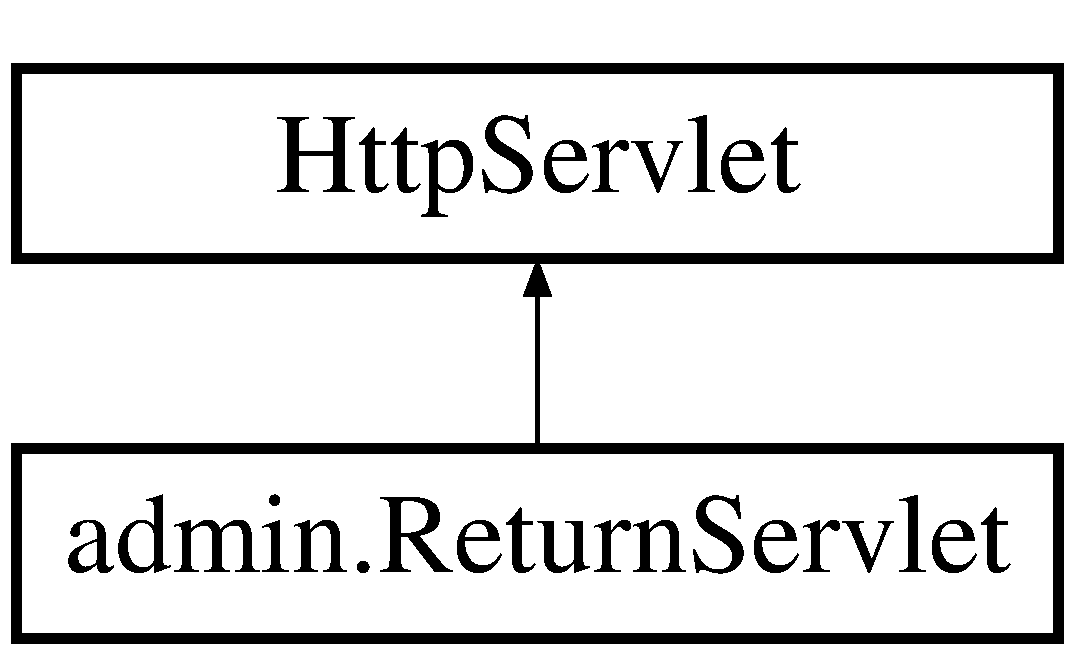
\includegraphics[height=2.000000cm]{classadmin_1_1_return_servlet}
\end{center}
\end{figure}
\subsection*{Public Member Functions}
\begin{DoxyCompactItemize}
\item 
\hyperlink{classadmin_1_1_return_servlet_a855b49f16845178a877261f45279927c}{Return\+Servlet} ()
\end{DoxyCompactItemize}
\subsection*{Protected Member Functions}
\begin{DoxyCompactItemize}
\item 
void \hyperlink{classadmin_1_1_return_servlet_a05243ac40e544c80bebc6ccc3af310e3}{do\+Get} (Http\+Servlet\+Request request, Http\+Servlet\+Response response)  throws Servlet\+Exception, I\+O\+Exception 
\item 
void \hyperlink{classadmin_1_1_return_servlet_af2c1e5273df5b6516d9e5f2c61b26eff}{do\+Post} (Http\+Servlet\+Request request, Http\+Servlet\+Response response)  throws Servlet\+Exception, I\+O\+Exception 
\end{DoxyCompactItemize}


\subsection{Detailed Description}
Servlet implementation class \hyperlink{classadmin_1_1_return_servlet}{Return\+Servlet} 

\subsection{Constructor \& Destructor Documentation}
\index{admin\+::\+Return\+Servlet@{admin\+::\+Return\+Servlet}!Return\+Servlet@{Return\+Servlet}}
\index{Return\+Servlet@{Return\+Servlet}!admin\+::\+Return\+Servlet@{admin\+::\+Return\+Servlet}}
\subsubsection[{\texorpdfstring{Return\+Servlet()}{ReturnServlet()}}]{\setlength{\rightskip}{0pt plus 5cm}admin.\+Return\+Servlet.\+Return\+Servlet (
\begin{DoxyParamCaption}
{}
\end{DoxyParamCaption}
)}\hypertarget{classadmin_1_1_return_servlet_a855b49f16845178a877261f45279927c}{}\label{classadmin_1_1_return_servlet_a855b49f16845178a877261f45279927c}
\begin{DoxySeeAlso}{See also}
Http\+Servlet\+::\+Http\+Servlet() 
\end{DoxySeeAlso}


\subsection{Member Function Documentation}
\index{admin\+::\+Return\+Servlet@{admin\+::\+Return\+Servlet}!do\+Get@{do\+Get}}
\index{do\+Get@{do\+Get}!admin\+::\+Return\+Servlet@{admin\+::\+Return\+Servlet}}
\subsubsection[{\texorpdfstring{do\+Get(\+Http\+Servlet\+Request request, Http\+Servlet\+Response response)}{doGet(HttpServletRequest request, HttpServletResponse response)}}]{\setlength{\rightskip}{0pt plus 5cm}void admin.\+Return\+Servlet.\+do\+Get (
\begin{DoxyParamCaption}
\item[{Http\+Servlet\+Request}]{request, }
\item[{Http\+Servlet\+Response}]{response}
\end{DoxyParamCaption}
) throws Servlet\+Exception, I\+O\+Exception\hspace{0.3cm}{\ttfamily [protected]}}\hypertarget{classadmin_1_1_return_servlet_a05243ac40e544c80bebc6ccc3af310e3}{}\label{classadmin_1_1_return_servlet_a05243ac40e544c80bebc6ccc3af310e3}
\begin{DoxySeeAlso}{See also}
Http\+Servlet\+::do\+Get(\+Http\+Servlet\+Request request, Http\+Servlet\+Response response) 
\end{DoxySeeAlso}
\index{admin\+::\+Return\+Servlet@{admin\+::\+Return\+Servlet}!do\+Post@{do\+Post}}
\index{do\+Post@{do\+Post}!admin\+::\+Return\+Servlet@{admin\+::\+Return\+Servlet}}
\subsubsection[{\texorpdfstring{do\+Post(\+Http\+Servlet\+Request request, Http\+Servlet\+Response response)}{doPost(HttpServletRequest request, HttpServletResponse response)}}]{\setlength{\rightskip}{0pt plus 5cm}void admin.\+Return\+Servlet.\+do\+Post (
\begin{DoxyParamCaption}
\item[{Http\+Servlet\+Request}]{request, }
\item[{Http\+Servlet\+Response}]{response}
\end{DoxyParamCaption}
) throws Servlet\+Exception, I\+O\+Exception\hspace{0.3cm}{\ttfamily [protected]}}\hypertarget{classadmin_1_1_return_servlet_af2c1e5273df5b6516d9e5f2c61b26eff}{}\label{classadmin_1_1_return_servlet_af2c1e5273df5b6516d9e5f2c61b26eff}
\begin{DoxySeeAlso}{See also}
Http\+Servlet\+::do\+Post(\+Http\+Servlet\+Request request, Http\+Servlet\+Response response) 
\end{DoxySeeAlso}


The documentation for this class was generated from the following file\+:\begin{DoxyCompactItemize}
\item 
Return\+Servlet.\+java\end{DoxyCompactItemize}

\hypertarget{classadmin_1_1_search_servlet}{}\section{admin.\+Search\+Servlet Class Reference}
\label{classadmin_1_1_search_servlet}\index{admin.\+Search\+Servlet@{admin.\+Search\+Servlet}}
Inheritance diagram for admin.\+Search\+Servlet\+:\begin{figure}[H]
\begin{center}
\leavevmode
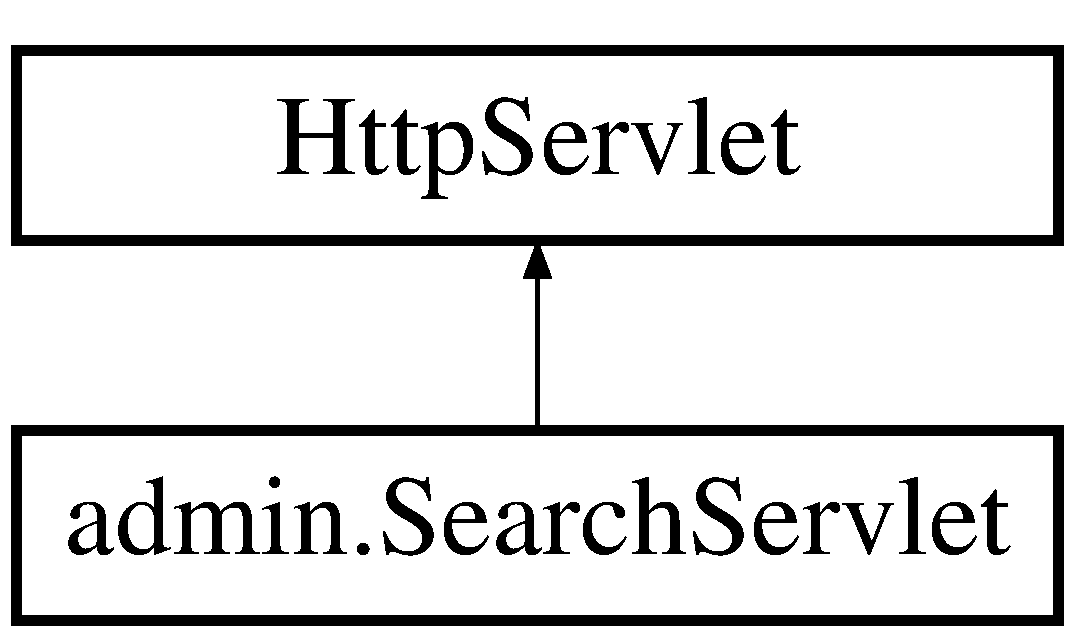
\includegraphics[height=2.000000cm]{classadmin_1_1_search_servlet}
\end{center}
\end{figure}
\subsection*{Public Member Functions}
\begin{DoxyCompactItemize}
\item 
\hyperlink{classadmin_1_1_search_servlet_ab50b346d5eff83597546471d03831aa5}{Search\+Servlet} ()
\end{DoxyCompactItemize}
\subsection*{Static Public Member Functions}
\begin{DoxyCompactItemize}
\item 
static void {\bfseries main} (String\mbox{[}$\,$\mbox{]} args)\hypertarget{classadmin_1_1_search_servlet_a28154723497a97fdf737746ffdf234e8}{}\label{classadmin_1_1_search_servlet_a28154723497a97fdf737746ffdf234e8}

\end{DoxyCompactItemize}
\subsection*{Protected Member Functions}
\begin{DoxyCompactItemize}
\item 
void \hyperlink{classadmin_1_1_search_servlet_af33243d76918c14089eccbc1ca0fbf3a}{do\+Get} (Http\+Servlet\+Request request, Http\+Servlet\+Response response)  throws Servlet\+Exception, I\+O\+Exception 
\item 
void \hyperlink{classadmin_1_1_search_servlet_a9183bb5f24ea47c4b159e836e84990d8}{do\+Post} (Http\+Servlet\+Request request, Http\+Servlet\+Response response)  throws Servlet\+Exception, I\+O\+Exception 
\end{DoxyCompactItemize}


\subsection{Detailed Description}
Servlet implementation class \hyperlink{classadmin_1_1_search_servlet}{Search\+Servlet} 

\subsection{Constructor \& Destructor Documentation}
\index{admin\+::\+Search\+Servlet@{admin\+::\+Search\+Servlet}!Search\+Servlet@{Search\+Servlet}}
\index{Search\+Servlet@{Search\+Servlet}!admin\+::\+Search\+Servlet@{admin\+::\+Search\+Servlet}}
\subsubsection[{\texorpdfstring{Search\+Servlet()}{SearchServlet()}}]{\setlength{\rightskip}{0pt plus 5cm}admin.\+Search\+Servlet.\+Search\+Servlet (
\begin{DoxyParamCaption}
{}
\end{DoxyParamCaption}
)}\hypertarget{classadmin_1_1_search_servlet_ab50b346d5eff83597546471d03831aa5}{}\label{classadmin_1_1_search_servlet_ab50b346d5eff83597546471d03831aa5}
\begin{DoxySeeAlso}{See also}
Http\+Servlet\+::\+Http\+Servlet() 
\end{DoxySeeAlso}


\subsection{Member Function Documentation}
\index{admin\+::\+Search\+Servlet@{admin\+::\+Search\+Servlet}!do\+Get@{do\+Get}}
\index{do\+Get@{do\+Get}!admin\+::\+Search\+Servlet@{admin\+::\+Search\+Servlet}}
\subsubsection[{\texorpdfstring{do\+Get(\+Http\+Servlet\+Request request, Http\+Servlet\+Response response)}{doGet(HttpServletRequest request, HttpServletResponse response)}}]{\setlength{\rightskip}{0pt plus 5cm}void admin.\+Search\+Servlet.\+do\+Get (
\begin{DoxyParamCaption}
\item[{Http\+Servlet\+Request}]{request, }
\item[{Http\+Servlet\+Response}]{response}
\end{DoxyParamCaption}
) throws Servlet\+Exception, I\+O\+Exception\hspace{0.3cm}{\ttfamily [protected]}}\hypertarget{classadmin_1_1_search_servlet_af33243d76918c14089eccbc1ca0fbf3a}{}\label{classadmin_1_1_search_servlet_af33243d76918c14089eccbc1ca0fbf3a}
\begin{DoxySeeAlso}{See also}
Http\+Servlet\+::do\+Get(\+Http\+Servlet\+Request request, Http\+Servlet\+Response response) 
\end{DoxySeeAlso}
\index{admin\+::\+Search\+Servlet@{admin\+::\+Search\+Servlet}!do\+Post@{do\+Post}}
\index{do\+Post@{do\+Post}!admin\+::\+Search\+Servlet@{admin\+::\+Search\+Servlet}}
\subsubsection[{\texorpdfstring{do\+Post(\+Http\+Servlet\+Request request, Http\+Servlet\+Response response)}{doPost(HttpServletRequest request, HttpServletResponse response)}}]{\setlength{\rightskip}{0pt plus 5cm}void admin.\+Search\+Servlet.\+do\+Post (
\begin{DoxyParamCaption}
\item[{Http\+Servlet\+Request}]{request, }
\item[{Http\+Servlet\+Response}]{response}
\end{DoxyParamCaption}
) throws Servlet\+Exception, I\+O\+Exception\hspace{0.3cm}{\ttfamily [protected]}}\hypertarget{classadmin_1_1_search_servlet_a9183bb5f24ea47c4b159e836e84990d8}{}\label{classadmin_1_1_search_servlet_a9183bb5f24ea47c4b159e836e84990d8}
\begin{DoxySeeAlso}{See also}
Http\+Servlet\+::do\+Post(\+Http\+Servlet\+Request request, Http\+Servlet\+Response response) 
\end{DoxySeeAlso}


The documentation for this class was generated from the following file\+:\begin{DoxyCompactItemize}
\item 
Search\+Servlet.\+java\end{DoxyCompactItemize}

%--- End generated contents ---

% Index
\backmatter
\newpage
\phantomsection
\clearemptydoublepage
\addcontentsline{toc}{chapter}{Index}
\printindex

\end{document}
